% Options for packages loaded elsewhere
\PassOptionsToPackage{unicode}{hyperref}
\PassOptionsToPackage{hyphens}{url}
\documentclass[11pt,a4paper]{article}
\usepackage{xcolor}
\usepackage{amsmath,amssymb}
\setcounter{secnumdepth}{-1}
\usepackage{iftex}
\ifPDFTeX
  \usepackage[T1]{fontenc}
  \usepackage[utf8]{inputenc}
  \usepackage{textcomp} % provide euro and other symbols
\else % if luatex or xetex
  \usepackage{unicode-math} % this also loads fontspec
  \defaultfontfeatures{Scale=MatchLowercase}
  \defaultfontfeatures[\rmfamily]{Ligatures=TeX,Scale=1}
\fi
\ifPDFTeX
  \usepackage{lmodern}
\else
  \setmainfont{Libertinus Serif}
  \setsansfont{Libertinus Sans}
  \setmonofont[Scale=0.78]{DejaVu Sans Mono}
  \setmathfont{Libertinus Math}
\fi
% Use upquote if available, for straight quotes in verbatim environments
\IfFileExists{upquote.sty}{\usepackage{upquote}}{}
\IfFileExists{microtype.sty}{% use microtype if available
  \usepackage[]{microtype}
  \UseMicrotypeSet[protrusion]{basicmath} % disable protrusion for tt fonts
}{}
\makeatletter
\@ifundefined{KOMAClassName}{% if non-KOMA class
  \IfFileExists{parskip.sty}{%
    \usepackage{parskip}
  }{% else
    \setlength{\parindent}{0pt}
    \setlength{\parskip}{6pt plus 2pt minus 1pt}}
}{% if KOMA class
  \KOMAoptions{parskip=half}}
\makeatother
\usepackage{color}
\usepackage{fvextra}
\newcommand{\VerbBar}{|}
\newcommand{\VERB}{\Verb[commandchars=\\\{\}]}
\DefineVerbatimEnvironment{Highlighting}{Verbatim}{commandchars=\\\{\},fontsize=\small,breaklines=true,breakanywhere=true}
% Add ',fontsize=\small' for more characters per line
\newenvironment{Shaded}{}{}
\newcommand{\AlertTok}[1]{\textcolor[rgb]{1.00,0.00,0.00}{\textbf{#1}}}
\newcommand{\AnnotationTok}[1]{\textcolor[rgb]{0.38,0.63,0.69}{\textbf{\textit{#1}}}}
\newcommand{\AttributeTok}[1]{\textcolor[rgb]{0.49,0.56,0.16}{#1}}
\newcommand{\BaseNTok}[1]{\textcolor[rgb]{0.25,0.63,0.44}{#1}}
\newcommand{\BuiltInTok}[1]{\textcolor[rgb]{0.00,0.50,0.00}{#1}}
\newcommand{\CharTok}[1]{\textcolor[rgb]{0.25,0.44,0.63}{#1}}
\newcommand{\CommentTok}[1]{\textcolor[rgb]{0.38,0.63,0.69}{\textit{#1}}}
\newcommand{\CommentVarTok}[1]{\textcolor[rgb]{0.38,0.63,0.69}{\textbf{\textit{#1}}}}
\newcommand{\ConstantTok}[1]{\textcolor[rgb]{0.53,0.00,0.00}{#1}}
\newcommand{\ControlFlowTok}[1]{\textcolor[rgb]{0.00,0.44,0.13}{\textbf{#1}}}
\newcommand{\DataTypeTok}[1]{\textcolor[rgb]{0.56,0.13,0.00}{#1}}
\newcommand{\DecValTok}[1]{\textcolor[rgb]{0.25,0.63,0.44}{#1}}
\newcommand{\DocumentationTok}[1]{\textcolor[rgb]{0.73,0.13,0.13}{\textit{#1}}}
\newcommand{\ErrorTok}[1]{\textcolor[rgb]{1.00,0.00,0.00}{\textbf{#1}}}
\newcommand{\ExtensionTok}[1]{#1}
\newcommand{\FloatTok}[1]{\textcolor[rgb]{0.25,0.63,0.44}{#1}}
\newcommand{\FunctionTok}[1]{\textcolor[rgb]{0.02,0.16,0.49}{#1}}
\newcommand{\ImportTok}[1]{\textcolor[rgb]{0.00,0.50,0.00}{\textbf{#1}}}
\newcommand{\InformationTok}[1]{\textcolor[rgb]{0.38,0.63,0.69}{\textbf{\textit{#1}}}}
\newcommand{\KeywordTok}[1]{\textcolor[rgb]{0.00,0.44,0.13}{\textbf{#1}}}
\newcommand{\NormalTok}[1]{#1}
\newcommand{\OperatorTok}[1]{\textcolor[rgb]{0.40,0.40,0.40}{#1}}
\newcommand{\OtherTok}[1]{\textcolor[rgb]{0.00,0.44,0.13}{#1}}
\newcommand{\PreprocessorTok}[1]{\textcolor[rgb]{0.74,0.48,0.00}{#1}}
\newcommand{\RegionMarkerTok}[1]{#1}
\newcommand{\SpecialCharTok}[1]{\textcolor[rgb]{0.25,0.44,0.63}{#1}}
\newcommand{\SpecialStringTok}[1]{\textcolor[rgb]{0.73,0.40,0.53}{#1}}
\newcommand{\StringTok}[1]{\textcolor[rgb]{0.25,0.44,0.63}{#1}}
\newcommand{\VariableTok}[1]{\textcolor[rgb]{0.10,0.09,0.49}{#1}}
\newcommand{\VerbatimStringTok}[1]{\textcolor[rgb]{0.25,0.44,0.63}{#1}}
\newcommand{\WarningTok}[1]{\textcolor[rgb]{0.38,0.63,0.69}{\textbf{\textit{#1}}}}
\usepackage{longtable,booktabs,array}
\usepackage[a4paper,margin=2.35cm,headheight=14pt]{geometry}
\usepackage[spanish,es-nodecimaldot,es-noshorthands]{babel}
\usepackage{graphicx}
\usepackage{float}
\usepackage{pdflscape}
\usepackage{tikz}
\usetikzlibrary{arrows.meta,fit,positioning,shapes.geometric}
\usepackage{fancyhdr}
\usepackage{caption}
\usepackage{enumitem}
\usepackage{csquotes}
\newcolumntype{L}[1]{>{\raggedright\arraybackslash}p{#1}}
\newcolumntype{C}[1]{>{\centering\arraybackslash}p{#1}}
\usepackage{calc} % for calculating minipage widths
% Correct order of tables after \paragraph or \subparagraph
\usepackage{etoolbox}
\makeatletter
\patchcmd\longtable{\par}{\if@noskipsec\mbox{}\fi\par}{}{}
\makeatother
% Allow footnotes in longtable head/foot
\IfFileExists{footnotehyper.sty}{\usepackage{footnotehyper}}{\usepackage{footnote}}
\makesavenoteenv{longtable}
\setlength{\emergencystretch}{3em} % prevent overfull lines
\AtBeginEnvironment{longtable}{\fontsize{7}{8}\selectfont\setlength{\tabcolsep}{2pt}}
\providecommand{\tightlist}{%
  \setlength{\itemsep}{0pt}\setlength{\parskip}{0pt}}
\usepackage{bookmark}
\IfFileExists{xurl.sty}{\usepackage{xurl}}{} % add URL line breaks if available
\urlstyle{same}
\hypersetup{
  colorlinks=true,
  linkcolor=blue!45!black,
  urlcolor=blue!55!black,
  citecolor=blue!45!black,
  pdftitle={Integración de búsqueda exacta por similitud vectorial en un Mini-SGBD paginado},
  pdfauthor={Javier Alonzo Peñalva Humire; Lizzy Arlette Huayhua Perez; Emilio Alejandro Condori Pallardel},
  pdfcreator={LuaLaTeX}}

\definecolor{unsaBlue}{HTML}{17365D}
\definecolor{vectorBlue}{HTML}{E8F1FA}
\captionsetup{font=small,labelfont=bf}
\setlist{nosep,leftmargin=*}
\pagestyle{fancy}
\fancyhf{}
\fancyhead[L]{\small Búsqueda exacta por similitud vectorial en un Mini-SGBD}
\fancyhead[R]{\small Universidad Nacional de San Agustín}
\fancyfoot[C]{\thepage}
\renewcommand{\headrulewidth}{0.4pt}
\let\pandocsubsection\subsection
\let\pandocsubsubsection\subsubsection
\let\subsection\section
\let\subsubsection\pandocsubsection
\title{\bfseries\color{unsaBlue}Integración de búsqueda exacta por similitud vectorial en un Mini-SGBD paginado:\\[0.35em]
\large Selección Top-k acotada frente a ordenamiento completo}
\author{Javier Alonzo Peñalva Humire\\\texttt{jpenalvah@unsa.edu.pe}
\and Lizzy Arlette Huayhua Perez\\\texttt{lhuayhuape@unsa.edu.pe}
\and Emilio Alejandro Condori Pallardel\\\texttt{econdoripal@unsa.edu.pe}}
\date{\small Escuela Profesional de Ciencia de la Computación\\
Universidad Nacional de San Agustín de Arequipa\\Arequipa, Perú\\[0.5em]
Curso: Base de Datos II \quad Docente: \textbf{[COMPLETAR NOMBRE DEL DOCENTE]}}

\begin{document}

\maketitle
\thispagestyle{empty}

\section*{Resumen}\label{resumen}

Los sistemas gestores de bases de datos relacionales recuperan registros
mediante predicados de igualdad y orden sobre valores escalares, un
modelo que no expresa la noción de proximidad que requieren las
representaciones vectoriales densas. Este trabajo incorpora búsqueda por
similitud vectorial a un Sistema Gestor de Base de Datos (SGBD)
didáctico escrito en C++20, con almacenamiento paginado, administrador
de buffer con reemplazo LRU (\emph{Least Recently Used}) y procesamiento
de consultas según el modelo Volcano. El aporte es un tipo de dato
vectorial persistido en las mismas páginas ranuradas que los registros
convencionales, tres funciones de distancia y similitud, y una consulta
de los \texttt{k} vecinos más cercanos integrada en la gramática del
sistema. Se comparan dos estrategias de ranking, ambas exactas y
exhaustivas: una selección Top-k mediante montículo acotado y un
ordenamiento completo de las \texttt{n} distancias, cuyos costes son
\texttt{O(n·d\ +\ n\ log\ k)} y \texttt{O(n·d\ +\ n\ log\ n)}. Sobre
vectores sintéticos con semilla fija, de 1000 a 100 000 vectores,
dimensiones de 16 a 256 y \texttt{k} entre 1 y 50, se midieron latencia,
percentiles, distancias calculadas y métricas del buffer, con 30
consultas por configuración. La selección Top-k reduce la latencia entre
1,19 y 1,67 veces, con una ventaja que crece con el número de vectores y
decrece con la dimensionalidad, mientras el coste de entrada y salida
resulta idéntico en ambas. La limitación principal es que la búsqueda
permanece exhaustiva: sin índice vectorial, el coste sigue siendo lineal
en el número de vectores almacenados.

\paragraph{Palabras clave.}

Mini-SGBD; búsqueda por similitud vectorial; vecinos más cercanos;
selección Top-k; distancia euclidiana; similitud coseno; administración
de buffer; modelo Volcano.

\vspace{0.6em}\hrule\vspace{1em}

\subsection{1. Introducción}\label{1-introducciuxf3n}

Los sistemas gestores de bases de datos (SGBD) organizan la información
en estructuras que permiten recuperarla mediante predicados sobre
valores escalares. Los métodos de acceso clásicos ---índices basados en
árboles B+ y en tablas de dispersión--- están diseñados para responder
preguntas de igualdad y de rango sobre dominios totalmente ordenados.
Esa correspondencia entre el predicado y la estructura de acceso es la
que permite que una consulta sobre millones de registros se resuelva
tocando unas pocas páginas.

El crecimiento de los datos no estructurados ha desplazado parte de la
carga de consulta hacia un tipo de pregunta que ese modelo no expresa.
Textos, imágenes y audio se representan hoy mediante vectores densos de
decenas o cientos de dimensiones, obtenidos de modelos de aprendizaje
profundo, en los que la proximidad geométrica aproxima la similitud
semántica. La pregunta relevante deja de ser «qué registros tienen
exactamente este valor» y pasa a ser «qué registros se parecen más a
este». Un índice hash no puede responderla: dispersa las claves
precisamente para destruir la vecindad, de modo que dos vectores casi
idénticos caen en cubetas sin relación. Un árbol B+ tampoco, porque un
vector de dimensión \texttt{d\ \textgreater{}\ 1} no admite un orden
total único que preserve la proximidad en todas las direcciones.

Esta brecha ha producido una generación de sistemas especializados y de
extensiones a sistemas existentes. El problema, sin embargo, no es
solamente de estructura de índice: incorporar vectores a un SGBD exige
decidir cómo se representan en el formato binario, cómo se validan, cómo
se relacionan con los registros convencionales y cómo se integra el
operador de ranking en el motor de consultas existente. Esas decisiones
son las que este trabajo aborda.

\textbf{Problema abordado.} Un SGBD didáctico con almacenamiento
paginado, administrador de buffer y procesamiento de consultas por
operadores físicos no puede expresar ni resolver consultas de
proximidad, porque su sistema de tipos no representa vectores y su único
método de acceso responde igualdades exactas.

\textbf{Objetivo.} Incorporar búsqueda exacta por similitud vectorial al
sistema, integrada con su gestor de almacenamiento, su administrador de
buffer y su modelo de ejecución, y evaluar cuantitativamente el efecto
de la estrategia de ranking sobre el coste de la consulta.

\textbf{Alcance.} El trabajo cubre la representación, la persistencia,
las métricas, la consulta de los \texttt{k} vecinos más cercanos y su
evaluación experimental. \textbf{No} cubre la construcción de un índice
vectorial: la búsqueda implementada es exhaustiva, y el artículo es
explícito al respecto en cada punto donde podría confundirse. La
búsqueda aproximada y, con ella, la métrica \texttt{Recall@k}, quedan
fuera por la misma razón.

\textbf{Aporte distintivo.} Dentro del contexto del proyecto, la
contribución es la integración de un tipo de dato vectorial y de una
consulta de vecinos más cercanos en un motor paginado preexistente,
junto con la comparación medida de dos estrategias de ranking sobre
datos, consultas y configuración idénticos. No se reclama novedad
científica frente a la literatura de búsqueda vectorial: los algoritmos
empleados son conocidos, y lo que el trabajo aporta es su integración
verificable y su evaluación en un sistema cuyo comportamiento de entrada
y salida es observable en detalle.

\textbf{Limitaciones principales.} El coste de una consulta crece
linealmente con el número de vectores almacenados; la mejora obtenida es
un factor constante, no un cambio de orden de complejidad; y los
volúmenes evaluados están acotados por el formato de página de 4 KiB del
sistema.

\subsubsection{1.1 Contribuciones
verificables}\label{11-contribuciones-verificables}

\begin{enumerate}
\def\labelenumi{\arabic{enumi}.}
\tightlist
\item
  Un tipo de dato \texttt{VECTOR(d)} con dimensión fija declarada en el
  esquema, serializado en formato IEEE 754 binario de 32 bits
  \emph{little-endian} y persistido en las mismas páginas ranuradas que
  los demás registros (\texttt{src/storage/record.cpp}, funciones
  \texttt{Record::SerializeTo} y \texttt{Record::DeserializeFrom}).
\item
  La restauración de un invariante del diseño original que el tipo
  vectorial rompía: la garantía de que ningún registro válido puede
  exceder la capacidad de una página vacía
  (\texttt{src/catalog/schema.cpp}, constructor
  \texttt{Schema::Schema}).
\item
  Tres métricas ---distancia euclidiana, similitud y distancia coseno, y
  producto punto--- con tratamiento explícito del vector nulo y
  validación de dimensiones (\texttt{src/vector/distance.cpp}).
\item
  Dos operadores físicos que resuelven la misma consulta de vecinos más
  cercanos con costes de ranking distintos, y cuya equivalencia de
  resultados se verifica automáticamente
  (\texttt{src/execution/knn\_operators.cpp}).
\item
  Instrumentación de distancias calculadas y de candidatos retenidos,
  integrada en el mismo mecanismo de contadores por operador que el
  resto del motor
  (\texttt{include/minidb/execution/physical\_operator.hpp}).
\item
  Un arnés experimental reproducible con semilla fija, que exporta
  resultados crudos a CSV sin intervención manual
  (\texttt{experimentos/scripts/}).
\end{enumerate}

\subsubsection{1.2 Organización del
artículo}\label{12-organizaciuxf3n-del-artuxedculo}

La sección 2 sitúa el trabajo frente a la literatura de búsqueda por
similitud. La sección 3 describe la arquitectura del sistema y el punto
de integración del aporte. La sección 4 justifica las decisiones de
diseño y sus costes teóricos. La sección 5 detalla la implementación con
referencias al código. La sección 6 presenta el diseño experimental y
los resultados. La sección 7 los interpreta y discute sus amenazas a la
validez. La sección 8 concluye y propone trabajo futuro.

\begin{center}\rule{0.5\linewidth}{0.5pt}\end{center}

\subsection{2. Trabajos relacionados}\label{2-trabajos-relacionados}

\subsubsection{2.1 El problema de los vecinos más cercanos y el efecto
de la
dimensionalidad}\label{21-el-problema-de-los-vecinos-muxe1s-cercanos-y-el-efecto-de-la-dimensionalidad}

Dado un conjunto de vectores \texttt{V\ =\ \{v₁,\ …,\ vₙ\}} con
\texttt{vᵢ\ ∈\ ℝᵈ} y una consulta \texttt{q\ ∈\ ℝᵈ}, la búsqueda de los
\texttt{k} vecinos más cercanos consiste en obtener el subconjunto de
tamaño \texttt{k} que minimiza una función de distancia
\texttt{d(q,\ vᵢ)}, o que maximiza una función de similitud
\texttt{s(q,\ vᵢ)}.

La solución exacta por excelencia es el recorrido exhaustivo: calcular
las \texttt{n} distancias y seleccionar las \texttt{k} menores, con
coste \texttt{Θ(n·d)} en aritmética. Las estructuras de indexación
espacial clásicas ---árboles k-d {[}1{]} y árboles R {[}2{]}--- reducen
ese coste particionando el espacio, y funcionan bien en dimensiones
bajas.

El resultado que gobierna este campo es que dejan de funcionar al crecer
\texttt{d}. Weber, Schek y Blott {[}3{]} mostraron cuantitativamente
que, por encima de unas pocas decenas de dimensiones, cualquier método
de partición del espacio termina examinando una fracción tan grande del
conjunto que resulta más lento que un recorrido secuencial bien
implementado, porque el recorrido lee memoria de forma contigua y el
índice no. Beyer y colaboradores {[}4{]} complementaron ese análisis
mostrando que, bajo condiciones amplias, al crecer la dimensión la
distancia al vecino más cercano y la distancia al más lejano convergen,
de modo que la noción misma de «vecino más cercano» pierde contraste.

Esta es la razón por la que el recorrido exhaustivo sigue siendo una
línea base respetable en la literatura y no un método ingenuo, y por la
que el presente trabajo puede evaluar seriamente dos variantes de
ranking exhaustivo. Es también la razón por la que el campo se desplazó
hacia la búsqueda aproximada.

\subsubsection{2.2 Búsqueda aproximada}\label{22-buxfasqueda-aproximada}

La búsqueda aproximada renuncia a garantizar el resultado exacto para
obtener una reducción de latencia de órdenes de magnitud, y se evalúa
mediante \texttt{Recall@k}, la fracción de los \texttt{k} vecinos
verdaderos que recupera.

El \emph{hashing} sensible a la localidad (LSH) fue introducido por
Indyk y Motwani {[}5{]} y desarrollado para búsqueda en dimensiones
altas por Gionis, Indyk y Motwani {[}6{]}. Su idea es construir familias
de funciones que colisionen con probabilidad creciente en la proximidad:
exactamente lo contrario de la función hash que emplea un índice de
igualdad. Su ventaja es la garantía probabilística demostrable; su
limitación, que alcanzar un \texttt{recall} alto exige muchas tablas y
por tanto mucha memoria.

La cuantización de producto (PQ), de Jégou, Douze y Schmid {[}7{]},
descompone el espacio en subespacios y cuantiza cada uno por separado,
comprimiendo cada vector a unos pocos bytes y permitiendo calcular
distancias aproximadas mediante tablas precalculadas. Su ventaja es la
compresión; su limitación, la pérdida de precisión inherente a la
cuantización.

Los grafos de proximidad jerárquicos (HNSW), de Malkov y Yashunin
{[}8{]}, construyen un grafo navegable multinivel y buscan por descenso
codicioso. Constituyen hoy el punto de referencia práctico en tiempo de
consulta, con la contrapartida de un coste de construcción y un consumo
de memoria elevados, y de una estructura difícil de mantener bajo
actualizaciones. Los índices de archivo invertido (IVF), popularizados
por la biblioteca FAISS {[}9{]}, {[}10{]}, agrupan los vectores en
celdas mediante k-means y exploran solo las más cercanas a la consulta,
ofreciendo un compromiso ajustable mediante el número de celdas
exploradas.

La diferencia de todos ellos respecto de este trabajo es directa:
ninguno está implementado aquí. Se describen porque delimitan lo que el
sistema \textbf{no} hace y porque son la línea de trabajo futuro más
natural, en particular IVF, cuyo patrón de celdas persistidas en páginas
encaja con la arquitectura descrita en la sección 3.

\subsubsection{2.3 Bases de datos vectoriales y extensiones a SGBD
existentes}\label{23-bases-de-datos-vectoriales-y-extensiones-a-sgbd-existentes}

Milvus {[}11{]} representa la aproximación de sistema especializado: una
arquitectura diseñada alrededor del índice vectorial, con almacenamiento
y planificación propios. Su ventaja es el rendimiento a gran escala; su
limitación, que la integración con datos relacionales queda fuera del
sistema.

La aproximación complementaria consiste en extender un SGBD relacional.
La extensión \texttt{pgvector} {[}12{]} añade a PostgreSQL un tipo de
dato vectorial, operadores de distancia e índices IVF-Flat y HNSW,
reutilizando el gestor de almacenamiento, el registro de escritura
anticipada y el planificador del sistema anfitrión. Sistemas como Qdrant
{[}13{]} ocupan una posición intermedia, con filtrado por metadatos
integrado en el recorrido del índice.

El presente trabajo sigue conceptualmente la segunda aproximación
---extender un motor existente en lugar de construir uno
especializado--- pero en una escala didáctica y sin índice vectorial. La
comparación pertinente no es de rendimiento, que sería absurda, sino de
decisiones de integración: qué se necesita tocar en el sistema de tipos,
en el formato binario, en el catálogo y en el motor de consultas para
que una consulta de proximidad conviva con las consultas relacionales.

\subsubsection{2.4 Procesamiento de consultas y administración de
buffer}\label{24-procesamiento-de-consultas-y-administraciuxf3n-de-buffer}

El motor sobre el que se construye el aporte sigue el modelo Volcano de
Graefe {[}14{]}, {[}15{]}, en el que cada operador físico es un iterador
con las operaciones \texttt{Open}, \texttt{Next} y \texttt{Close}, y un
plan es un árbol que transmite tuplas hacia arriba. Los operadores
introducidos en este trabajo son operadores Volcano bloqueantes: no
pueden emitir su primera fila antes de haber examinado la última de su
entrada, igual que un ordenamiento.

La ejecución por lotes, o vectorizada en el sentido de MonetDB/X100
{[}16{]}, amortiza el coste de interpretación del plan procesando
bloques de tuplas. Conviene subrayar que ese sentido del término
\emph{vectorización} ---procesamiento por lotes de registros--- es
distinto del que da título a este artículo, que se refiere a la
similitud entre vectores numéricos como dato. El sistema evaluado
implementa ambos, y la sección 6 documenta que el ranking de vecinos
puede alimentarse desde el escaneo por lotes sin que el resultado
cambie.

La gestión del buffer sigue los principios sistematizados por Effelsberg
y Haerder {[}17{]}, y los conceptos de página, marco y política de
reemplazo se emplean con el significado que les dan los textos de
referencia del área {[}18{]}, {[}19{]}.

\begin{center}\rule{0.5\linewidth}{0.5pt}\end{center}

\subsection{3. Arquitectura propuesta}\label{3-arquitectura-propuesta}

El sistema es un SGBD monoproceso y monohilo que persiste toda la base
de datos en un único archivo binario dividido en páginas de 4096 bytes.
La figura 1 muestra sus capas y el punto de integración del aporte.

\begin{figure}[H]
\centering
\resizebox{\textwidth}{!}{%
\begin{tikzpicture}[
  box/.style={draw,rounded corners,align=center,minimum height=9mm,minimum width=25mm,fill=white},
  vec/.style={box,fill=vectorBlue,draw=unsaBlue,very thick},
  store/.style={draw,cylinder,shape border rotate=90,aspect=0.28,align=center,minimum height=12mm,minimum width=25mm,fill=gray!12},
  arrow/.style={-{Latex[length=2mm]},thick},node distance=7mm and 10mm]
\node[box] (cli) {Interfaz CLI\\\texttt{src/main.cpp}};
\node[box,right=of cli] (db) {Database\\fachada};
\node[box,right=of db] (parser) {Tokenizer\\y Parser};
\node[box,right=of parser] (engine) {ExecutionEngine\\plan físico};
\node[box,below=of engine] (projection) {ProjectionOperator};
\node[vec,below left=of projection] (topk) {KnnScanOperator\\montículo Top-k};
\node[vec,below right=of projection] (full) {KnnFullSortOperator\\orden completo};
\node[vec,below=of topk,xshift=19mm] (metrics) {Métricas vectoriales\\euclidiana, coseno, punto};
\node[box,below=of metrics] (scan) {FilterOperator opcional\\SequentialScanOperator};
\node[box,below=of scan] (heap) {TableHeap y TablePage\\páginas ranuradas};
\node[box,below=of heap] (buffer) {BufferPoolManager\\LRU y contadores};
\node[box,left=of buffer] (catalog) {Catalog y Schema\\tipo \texttt{VECTOR(d)}};
\node[box,right=of buffer] (disk) {DiskManager};
\node[store,right=of disk] (file) {archivo binario\\páginas de 4096 B};
\draw[arrow] (cli)--(db); \draw[arrow] (db)--(parser); \draw[arrow] (parser)--(engine);
\draw[arrow] (engine)--(projection); \draw[arrow] (projection)--(topk); \draw[arrow] (projection)--(full);
\draw[arrow] (topk)--(metrics); \draw[arrow] (full)--(metrics); \draw[arrow] (metrics)--(scan);
\draw[arrow] (scan)--(heap); \draw[arrow] (heap)--(buffer); \draw[arrow] (catalog)--(buffer);
\draw[arrow] (catalog)|-(engine); \draw[arrow] (buffer)--(disk); \draw[arrow] (disk)--(file);
\node[draw=unsaBlue,dashed,rounded corners,thick,fit=(topk)(full)(metrics),inner sep=4mm,
label={[unsaBlue]below:Similitud vectorial (aporte)}] {};
\end{tikzpicture}}
\caption{Arquitectura del sistema. Los componentes resaltados corresponden al aporte de similitud vectorial.}
\label{fig:arquitectura}
\end{figure}

\subsubsection{3.1 Componentes y punto de
integración}\label{31-componentes-y-punto-de-integraciuxf3n}

\begin{longtable}[]{@{}L{0.17\textwidth}L{0.41\textwidth}L{0.35\textwidth}@{}}
\toprule\noalign{}
Componente & Responsabilidad & Archivo \\
\midrule\noalign{}
\endhead
\bottomrule\noalign{}
\endlastfoot
Interfaz & Lectura de sentencias, presentación de resultados, órdenes
internas de medición & \texttt{src/main.cpp} \\
Procesador de comandos & Texto SQL a estructuras de datos puras &
\texttt{src/parser/tokenizer.cpp}, \texttt{src/parser/parser.cpp} \\
Catálogo & Esquema y punteros raíz, persistidos en la página 1 &
\texttt{src/catalog/catalog.cpp} \\
Gestor de tablas & Cadena de páginas ranuradas, operaciones por
identificador de registro & \texttt{src/storage/table\_heap.cpp} \\
Administrador de páginas & Vista ranurada sobre 4096 bytes; directorio
de ranuras y compactación & \texttt{src/storage/table\_page.cpp} \\
Administrador de buffer & Marcos en RAM, tabla de páginas, reemplazo
LRU, contadores & \texttt{src/buffer/buffer\_pool\_manager.cpp} \\
Gestor de almacenamiento & Lectura y escritura de páginas completas,
asignación de identificadores &
\texttt{src/storage/disk\_manager.cpp} \\
\textbf{Tipo vectorial} & \texttt{VECTOR(d)} como tercer tipo de columna
& \texttt{include/minidb/common/types.hpp},
\texttt{include/minidb/common/value.hpp} \\
\textbf{Módulo de métricas} & Distancias y similitudes entre vectores &
\texttt{src/vector/distance.cpp} \\
\textbf{Ejecutor k-NN} & Ranking exacto con selección Top-k &
\texttt{src/execution/knn\_operators.cpp} \\
\textbf{Línea base de ranking} & Ranking exacto con orden completo &
ídem, clase \texttt{KnnFullSortOperator} \\
Instrumentación & Contadores por operador y por sentencia &
\texttt{include/minidb/execution/physical\_operator.hpp} \\
\end{longtable}

Índice vectorial: no implementado. El único índice del sistema es una
tabla de dispersión sobre la clave primaria
(\texttt{src/index/hash\_index.cpp}), que resuelve igualdades exactas y
no participa en la búsqueda por similitud.

La integración es deliberadamente conservadora. Los vectores no viven en
un almacenamiento aparte: son valores de columna dentro de los mismos
registros ranurados, leídos y escritos a través del mismo administrador
de buffer que todo lo demás. En consecuencia, una consulta de proximidad
se beneficia de la administración de memoria existente y sus accesos
aparecen en los mismos contadores de aciertos y fallos, lo que hace su
coste de entrada y salida directamente observable.

\begin{center}\rule{0.5\linewidth}{0.5pt}\end{center}

\subsection{4. Diseño del sistema}\label{4-diseuxf1o-del-sistema}

\subsubsection{4.1 Representación de los
vectores}\label{41-representaciuxf3n-de-los-vectores}

Un valor vectorial es un arreglo de \texttt{float} de 32 bits de
longitud fija. La dimensión se declara en el esquema y se almacena en el
mismo campo de 16 bits que ya guardaba la longitud máxima de una columna
\texttt{VARCHAR}, lo que evita modificar la disposición de la página de
catálogo.

La elección de \texttt{float} en lugar de \texttt{double} reduce a la
mitad los bytes por vector. La precisión de un ranking de similitud está
limitada por el propio modelo que produjo el vector mucho antes que por
los 24 bits de mantisa de un \texttt{float}, y los sistemas de
referencia del área utilizan 32 bits por la misma razón.

\textbf{Formato en disco.} Una dimensión de 16 bits seguida de
\texttt{d} valores de 32 bits en orden \emph{little-endian}:
\texttt{2\ +\ 4d} bytes. Los bits del \texttt{float} se obtienen con
\texttt{std::bit\_cast}, no reinterpretando un puntero, de modo que el
formato queda definido por el estándar y no por la disposición que el
compilador dé a un \texttt{float}.

La dimensión se escribe aunque el esquema ya la fije. Es redundancia
deliberada: un registro puede leerse sin consultar el catálogo, y una
longitud corrupta se detecta al deserializar en lugar de producir un
vector silenciosamente desplazado.

\textbf{Validaciones.} La dimensión declarada debe estar entre 1 y 1000;
un valor insertado debe tener exactamente la dimensión declarada; una
columna vectorial no puede ser clave primaria, porque el índice hash
mapea claves de 32 bits; y una columna vectorial no admite comparación
de orden ni agrupamiento, porque un vector no posee un orden total
natural único.

\textbf{Capacidad de página.} Con solo \texttt{INT} y \texttt{VARCHAR},
las cotas del sistema demostraban que el registro más ancho posible
ocupaba \texttt{8\ ×\ (2\ +\ 255)\ =\ 2056} bytes, holgadamente por
debajo de los 4080 disponibles en una página vacía. Un vector rompe esa
garantía: dos columnas \texttt{VECTOR(1000)} requerirían 8004 bytes. El
diseño restaura el invariante comprobando en el constructor del esquema
que el registro más ancho posible no exceda la capacidad de la página.
La alternativa ---descubrirlo al insertar--- produciría una tabla en la
que ciertas filas no caben en ninguna página.

\subsubsection{4.2 Métricas}\label{42-muxe9tricas}

Sea \texttt{x,\ y\ ∈\ ℝᵈ}. Las tres métricas implementadas son:

\textbf{Distancia euclidiana.}

\begin{verbatim}
d_euclidiana(x, y) = √( Σᵢ (xᵢ − yᵢ)² )
\end{verbatim}

Interpreta la disimilitud como separación geométrica y es sensible a la
magnitud de los vectores. Coste \texttt{Θ(d)} en tiempo y \texttt{O(1)}
en espacio adicional. Orden ascendente: menor es más similar.

\textbf{Similitud coseno.}

\begin{verbatim}
s_cos(x, y) = (x · y) / (‖x‖ ‖y‖)
\end{verbatim}

Mide el ángulo entre los vectores e ignora sus magnitudes, lo que la
hace la métrica habitual para representaciones cuya norma no es
informativa. Recorrido \texttt{{[}−1,\ 1{]}}, orden descendente. Coste
\texttt{Θ(d)}.

\textbf{Distancia coseno.}

\begin{verbatim}
d_cos(x, y) = 1 − s_cos(x, y)
\end{verbatim}

Recorrido \texttt{{[}0,\ 2{]}}, orden ascendente. Es una cantidad
distinta de la similitud, y confundirlas invierte el ranking; el diseño
las mantiene como funciones separadas y la distinción se verifica en las
pruebas.

\textbf{Producto punto.}

\begin{verbatim}
s_dot(x, y) = Σᵢ xᵢ yᵢ
\end{verbatim}

Orden descendente. Coincide con la similitud coseno cuando ambos
vectores están normalizados; el sistema no normaliza automáticamente, de
modo que la equivalencia es responsabilidad de quien carga los datos.

\textbf{Vector nulo.} El coseno no está definido cuando alguna norma es
cero, porque el vector nulo no tiene dirección. La implementación define
la similitud como 0 en ese caso y lo documenta, en lugar de devolver un
\texttt{NaN} que haría que el resultado del ranking dependiera del orden
en que se visitaron los registros.

\textbf{Puntuación de ranking.} Para que un único operador implemente
las tres métricas con una sola comparación, el diseño introduce una
puntuación en la que \textbf{menor es siempre más cercano}: la distancia
euclidiana \textbf{al cuadrado}, la distancia coseno, y el producto
punto \textbf{negado}. La raíz cuadrada se aplica únicamente a los
\texttt{k} valores que se reportan, no a los \texttt{n} que se comparan:
es una función monótona creciente, de modo que no altera el orden, y
omitirla ahorra \texttt{n\ −\ k} llamadas a \texttt{sqrt} por consulta.

\subsubsection{\texorpdfstring{4.3 Algoritmo de los \texttt{k} vecinos
más
cercanos}{4.3 Algoritmo de los k vecinos más cercanos}}\label{43-algoritmo-de-los-k-vecinos-muxe1s-cercanos}

Ambas estrategias son exactas y examinan todos los registros. Difieren
en el ranking.

\textbf{Selección Top-k acotada.} Mantiene un montículo de máximos de
tamaño \texttt{k}, cuya raíz es el peor de los supervivientes. Un
candidato solo entra si mejora esa raíz.

\begin{verbatim}
Abrir():
    si k = 0: cerrar hijo y terminar          # respuesta vacía sin leer la tabla
    mientras el hijo produzca un registro:
        puntuación ← RankingScore(métrica, vector del registro, consulta)
        contar una distancia
        si |montículo| < k:
            insertar candidato
        si no, si candidato mejor que la raíz del montículo:
            extraer la raíz e insertar el candidato
    cerrar el hijo
    ordenar el montículo de forma ascendente

Siguiente():
    devolver el siguiente elemento del resultado, añadiendo la columna de distancia
\end{verbatim}

Coste: \texttt{Θ(n·d)} de aritmética, \texttt{O(n\ log\ k)} de
operaciones de montículo, \texttt{O(k)} de espacio.

\textbf{Ordenamiento completo (línea base).} Puntúa cada registro,
\textbf{conserva todos}, ordena las \texttt{n} puntuaciones y descarta
todo salvo las \texttt{k} primeras. Coste \texttt{Θ(n·d)} de aritmética,
\texttt{O(n\ log\ n)} de ordenamiento, \texttt{O(n)} de espacio. Con una
tabla grande el coste espacial es el más dañino de los dos, porque cada
candidato arrastra un registro completo con su vector.

\textbf{Desempates.} Dos registros a la misma distancia se ordenan por
clave primaria. Sin esa regla el resultado dependería del orden en que
el montículo hubiera desalojado candidatos, que a su vez depende de la
disposición física de las páginas: la consulta dejaría de ser
reproducible.

\textbf{Casos límite.} \texttt{k\ =\ 0} produce una respuesta vacía sin
recorrer la tabla; \texttt{k\ \textgreater{}\ n} devuelve los \texttt{n}
registros; una tabla vacía devuelve cero filas y cero distancias
calculadas; una dimensión incompatible entre la consulta y la columna se
rechaza al construir el plan, antes de leer una sola página.

\subsubsection{4.4 Integración con el
motor}\label{44-integraciuxf3n-con-el-motor}

El plan de una consulta de proximidad es
\texttt{Projection(\ Knn(\ Filter?\ (\ Scan\ )\ )\ )}. Dos consecuencias
se siguen de esa forma:

\begin{enumerate}
\def\labelenumi{\arabic{enumi}.}
\tightlist
\item
  \textbf{Búsqueda híbrida.} Una cláusula \texttt{WHERE} situada debajo
  del ranking reduce el conjunto de candidatos antes de que se calcule
  una sola distancia. La sección 6 documenta que con un filtro que deja
  pasar 50 de 400 registros se calculan exactamente 50 distancias.
\item
  \textbf{Independencia del método de acceso.} El ranking consume de un
  operador de escaneo cualquiera, de modo que el escaneo tupla a tupla y
  el escaneo por lotes pueden alimentarlo indistintamente sin que el
  resultado cambie.
\end{enumerate}

La columna de distancia se añade a la salida con el nombre
\texttt{distancia}, y la proyección puede descartarla como cualquier
otra columna.

\subsubsection{4.5 Compromisos de
diseño}\label{45-compromisos-de-diseuxf1o}

\begin{longtable}[]{@{}L{0.28\textwidth}L{0.25\textwidth}L{0.40\textwidth}@{}}
\toprule\noalign{}
Decisión & Alternativa descartada & Motivo \\
\midrule\noalign{}
\endhead
\bottomrule\noalign{}
\endlastfoot
Vectores dentro del registro & Almacenamiento vectorial separado &
Reutiliza páginas, buffer y catálogo; los accesos aparecen en los
contadores existentes \\
\texttt{float} de 32 bits & \texttt{double} de 64 bits & Mitad de bytes
por vector; la precisión del modelo limita antes \\
Dimensión fija por esquema & Dimensión libre por fila & Una distancia
solo está definida entre vectores de igual dimensión \\
Distancia euclidiana al cuadrado para ordenar & Distancia con raíz & La
raíz es monótona: \texttt{n\ −\ k} llamadas a \texttt{sqrt} evitadas por
consulta \\
Desempate por clave primaria & Orden de visita & Reproducibilidad del
resultado \\
Sin índice vectorial & IVF, HNSW & Fuera del alcance declarado; se
propone como trabajo futuro \\
\end{longtable}

\begin{center}\rule{0.5\linewidth}{0.5pt}\end{center}

\subsection{5. Implementación}\label{5-implementaciuxf3n}

\textbf{Lenguaje y compilación.} C++20 sin extensiones, compilado con
GCC 16.1.1 mediante CMake 4.4.1 y Ninja 1.13.2. La única dependencia
externa es GoogleTest 1.17 como paquete del sistema. El proyecto suma
7735 líneas de cabeceras y fuentes y 5304 de pruebas.

Los avisos del compilador activos incluyen
\texttt{-Wall\ -Wextra\ -Wpedantic\ -Wshadow\ -Wconversion\ -Wsign-conversion\ -Wnull-dereference};
la compilación en modo \texttt{Release} no produce ninguno.

\textbf{Tipo vectorial.} El valor de una columna se representa como una
variante que incorpora el arreglo de \texttt{float}:

\begin{Shaded}
\begin{Highlighting}[]
\KeywordTok{using}\NormalTok{ Vector }\OperatorTok{=} \BuiltInTok{std::}\NormalTok{vector}\OperatorTok{\textless{}}\DataTypeTok{float}\OperatorTok{\textgreater{};}
\KeywordTok{using}\NormalTok{ Value }\OperatorTok{=} \BuiltInTok{std::}\NormalTok{variant}\OperatorTok{\textless{}}\BuiltInTok{std::}\NormalTok{int32\_t}\OperatorTok{,} \BuiltInTok{std::}\NormalTok{string}\OperatorTok{,}\NormalTok{ Vector}\OperatorTok{,} \DataTypeTok{float}\OperatorTok{\textgreater{};}
\end{Highlighting}
\end{Shaded}

La cuarta alternativa, \texttt{float} escalar, nunca se persiste: ningún
tipo de columna se corresponde con ella. Existe para que la distancia
calculada viaje por el plan como cualquier otro valor, y
\texttt{Record::Validate} la rechaza, que es lo que la mantiene fuera
del archivo.

Fuente: \texttt{include/minidb/common/value.hpp}

\textbf{Serialización.} Los bits del \texttt{float} se obtienen sin
reinterpretar punteros:

\begin{Shaded}
\begin{Highlighting}[]
\DataTypeTok{void}\NormalTok{ WriteF32}\OperatorTok{(}\BuiltInTok{std::}\NormalTok{span}\OperatorTok{\textless{}}\BuiltInTok{std::}\NormalTok{byte}\OperatorTok{\textgreater{}}\NormalTok{ buffer}\OperatorTok{,} \BuiltInTok{std::}\NormalTok{size\_t offset}\OperatorTok{,} \DataTypeTok{float}\NormalTok{ value}\OperatorTok{)} \OperatorTok{\{}
    \KeywordTok{static\_assert}\OperatorTok{(}\KeywordTok{sizeof}\OperatorTok{(}\DataTypeTok{float}\OperatorTok{)} \OperatorTok{==} \KeywordTok{sizeof}\OperatorTok{(}\BuiltInTok{std::}\NormalTok{uint32\_t}\OperatorTok{),}
                  \StringTok{"el formato del archivo asume IEEE 754 binary32"}\OperatorTok{);}
\NormalTok{    WriteLittleEndian}\OperatorTok{(}\NormalTok{buffer}\OperatorTok{,}\NormalTok{ offset}\OperatorTok{,} \BuiltInTok{std::}\NormalTok{bit\_cast}\OperatorTok{\textless{}}\BuiltInTok{std::}\NormalTok{uint32\_t}\OperatorTok{\textgreater{}(}\NormalTok{value}\OperatorTok{),} \KeywordTok{sizeof}\OperatorTok{(}\NormalTok{value}\OperatorTok{));}
\OperatorTok{\}}
\end{Highlighting}
\end{Shaded}

Fuente: \texttt{src/common/serialization.cpp}, función
\texttt{serialization::WriteF32}

\textbf{Métrica.} La puntuación de ranking unifica el sentido del orden
de las tres métricas:

\begin{Shaded}
\begin{Highlighting}[]
\DataTypeTok{float}\NormalTok{ RankingScore}\OperatorTok{(}\NormalTok{DistanceMetric metric}\OperatorTok{,} \AttributeTok{const}\NormalTok{ Vector}\OperatorTok{\&}\NormalTok{ left}\OperatorTok{,} \AttributeTok{const}\NormalTok{ Vector}\OperatorTok{\&}\NormalTok{ right}\OperatorTok{)} \OperatorTok{\{}
    \ControlFlowTok{switch} \OperatorTok{(}\NormalTok{metric}\OperatorTok{)} \OperatorTok{\{}
        \ControlFlowTok{case}\NormalTok{ DistanceMetric}\OperatorTok{::}\NormalTok{kEuclidean}\OperatorTok{:}
            \ControlFlowTok{return}\NormalTok{ SquaredEuclideanDistance}\OperatorTok{(}\NormalTok{left}\OperatorTok{,}\NormalTok{ right}\OperatorTok{);}
        \ControlFlowTok{case}\NormalTok{ DistanceMetric}\OperatorTok{::}\NormalTok{kCosine}\OperatorTok{:}
            \ControlFlowTok{return}\NormalTok{ CosineDistance}\OperatorTok{(}\NormalTok{left}\OperatorTok{,}\NormalTok{ right}\OperatorTok{);}
        \ControlFlowTok{case}\NormalTok{ DistanceMetric}\OperatorTok{::}\NormalTok{kDotProduct}\OperatorTok{:}
            \ControlFlowTok{return} \OperatorTok{{-}}\NormalTok{DotProduct}\OperatorTok{(}\NormalTok{left}\OperatorTok{,}\NormalTok{ right}\OperatorTok{);}
    \OperatorTok{\}}
    \ControlFlowTok{throw}\NormalTok{ StorageError}\OperatorTok{(}\StringTok{"Métrica de distancia desconocida"}\OperatorTok{);}
\OperatorTok{\}}
\end{Highlighting}
\end{Shaded}

Fuente: \texttt{src/vector/distance.cpp}, función
\texttt{vector\_metrics::RankingScore}

Las sumas se acumulan en \texttt{double} y se devuelven como
\texttt{float}: con 1000 dimensiones un acumulador de 32 bits pierde
precisión por redondeo, y el coste adicional es despreciable frente al
tráfico de memoria de leer los vectores.

\textbf{Selector Top-k.} El núcleo del operador propuesto es la
comparación contra la raíz del montículo:

\begin{Shaded}
\begin{Highlighting}[]
\ControlFlowTok{if} \OperatorTok{(}\VariableTok{results\_}\OperatorTok{.}\NormalTok{size}\OperatorTok{()} \OperatorTok{\textless{}} \VariableTok{clause\_}\OperatorTok{.}\NormalTok{k}\OperatorTok{)} \OperatorTok{\{}
\NormalTok{    CountCandidate}\OperatorTok{();}
    \VariableTok{results\_}\OperatorTok{.}\NormalTok{push\_back}\OperatorTok{(}\BuiltInTok{std::}\NormalTok{move}\OperatorTok{(}\NormalTok{candidate}\OperatorTok{));}
    \BuiltInTok{std::}\NormalTok{push\_heap}\OperatorTok{(}\VariableTok{results\_}\OperatorTok{.}\NormalTok{begin}\OperatorTok{(),} \VariableTok{results\_}\OperatorTok{.}\NormalTok{end}\OperatorTok{(),}\NormalTok{ farther}\OperatorTok{);}
    \ControlFlowTok{continue}\OperatorTok{;}
\OperatorTok{\}}
\ControlFlowTok{if} \OperatorTok{(}\NormalTok{Closer}\OperatorTok{(}\NormalTok{candidate}\OperatorTok{,} \VariableTok{results\_}\OperatorTok{.}\NormalTok{front}\OperatorTok{()))} \OperatorTok{\{}
\NormalTok{    CountCandidate}\OperatorTok{();}
    \BuiltInTok{std::}\NormalTok{pop\_heap}\OperatorTok{(}\VariableTok{results\_}\OperatorTok{.}\NormalTok{begin}\OperatorTok{(),} \VariableTok{results\_}\OperatorTok{.}\NormalTok{end}\OperatorTok{(),}\NormalTok{ farther}\OperatorTok{);}
    \VariableTok{results\_}\OperatorTok{.}\NormalTok{back}\OperatorTok{()} \OperatorTok{=} \BuiltInTok{std::}\NormalTok{move}\OperatorTok{(}\NormalTok{candidate}\OperatorTok{);}
    \BuiltInTok{std::}\NormalTok{push\_heap}\OperatorTok{(}\VariableTok{results\_}\OperatorTok{.}\NormalTok{begin}\OperatorTok{(),} \VariableTok{results\_}\OperatorTok{.}\NormalTok{end}\OperatorTok{(),}\NormalTok{ farther}\OperatorTok{);}
\OperatorTok{\}}
\end{Highlighting}
\end{Shaded}

Fuente: \texttt{src/execution/knn\_operators.cpp}, función
\texttt{KnnScanOperator::Open}

\textbf{Línea base.} El ordenamiento completo comparte el cálculo de
puntuación y difiere solo en que conserva todos los candidatos y ordena
\texttt{n} elementos:

\begin{Shaded}
\begin{Highlighting}[]
\ControlFlowTok{while} \OperatorTok{(}\KeywordTok{auto}\NormalTok{ record }\OperatorTok{=} \VariableTok{child\_}\OperatorTok{{-}\textgreater{}}\NormalTok{Next}\OperatorTok{())} \OperatorTok{\{}
    \VariableTok{results\_}\OperatorTok{.}\NormalTok{push\_back}\OperatorTok{(}\NormalTok{Score}\OperatorTok{(}\BuiltInTok{std::}\NormalTok{move}\OperatorTok{(*}\NormalTok{record}\OperatorTok{)));}
\NormalTok{    CountCandidate}\OperatorTok{();}
\OperatorTok{\}}
\VariableTok{child\_}\OperatorTok{{-}\textgreater{}}\NormalTok{Close}\OperatorTok{();}
\BuiltInTok{std::}\NormalTok{sort}\OperatorTok{(}\VariableTok{results\_}\OperatorTok{.}\NormalTok{begin}\OperatorTok{(),} \VariableTok{results\_}\OperatorTok{.}\NormalTok{end}\OperatorTok{(),}\NormalTok{ Closer}\OperatorTok{);}
\ControlFlowTok{if} \OperatorTok{(}\VariableTok{results\_}\OperatorTok{.}\NormalTok{size}\OperatorTok{()} \OperatorTok{\textgreater{}} \VariableTok{clause\_}\OperatorTok{.}\NormalTok{k}\OperatorTok{)} \OperatorTok{\{}
    \VariableTok{results\_}\OperatorTok{.}\NormalTok{resize}\OperatorTok{(}\VariableTok{clause\_}\OperatorTok{.}\NormalTok{k}\OperatorTok{);}
\OperatorTok{\}}
\end{Highlighting}
\end{Shaded}

Fuente: \texttt{src/execution/knn\_operators.cpp}, función
\texttt{KnnFullSortOperator::Open}

Que ambas estrategias compartan la función \texttt{Score} no es un
detalle de estilo: es lo que garantiza que la aritmética medida sea
idéntica y que la diferencia observada proceda exclusivamente del
ranking.

\textbf{Contadores.} La instrumentación se incrementa en el punto exacto
donde ocurre el trabajo, de modo que no puede desviarse de él:

\begin{Shaded}
\begin{Highlighting}[]
\DataTypeTok{void}\NormalTok{ CountDistance}\OperatorTok{()} \OperatorTok{\{} \OperatorTok{++}\VariableTok{distance\_calculations\_}\OperatorTok{;} \OperatorTok{\}}
\DataTypeTok{void}\NormalTok{ CountCandidate}\OperatorTok{()} \OperatorTok{\{} \OperatorTok{++}\VariableTok{candidates\_admitted\_}\OperatorTok{;} \OperatorTok{\}}
\end{Highlighting}
\end{Shaded}

Fuente: \texttt{include/minidb/execution/physical\_operator.hpp}, clase
\texttt{PhysicalOperator}

\textbf{Contadores de buffer.} Los que ya existían distinguen las tres
nociones que el diseño experimental requiere: un acceso lógico se
contabiliza como acierto o fallo en
\texttt{BufferPoolManager::FetchPage}, mientras que \texttt{disk\_reads}
se incrementa únicamente cuando se invoca
\texttt{DiskManager::ReadPage}, es decir cuando hay lectura física.

Fuente: \texttt{src/buffer/buffer\_pool\_manager.cpp}, función
\texttt{BufferPoolManager::FetchPage}

\textbf{Interfaz de consulta.} La gramática admitida es:

\begin{Shaded}
\begin{Highlighting}[]
\KeywordTok{SELECT}\NormalTok{ \{ }\OperatorTok{*}\NormalTok{ | }\OperatorTok{\textless{}}\NormalTok{col}\OperatorTok{\textgreater{}}\NormalTok{ | }\FunctionTok{COUNT}\NormalTok{(}\OperatorTok{*}\NormalTok{) \}, }\OperatorTok{..}\NormalTok{. }\KeywordTok{FROM} \OperatorTok{\textless{}}\NormalTok{tabla}\OperatorTok{\textgreater{}}
\NormalTok{    [}\KeywordTok{WHERE} \OperatorTok{\textless{}}\NormalTok{col}\OperatorTok{\textgreater{}} \OperatorTok{\textless{}}\NormalTok{op}\OperatorTok{\textgreater{}} \OperatorTok{\textless{}}\NormalTok{valor}\OperatorTok{\textgreater{}}\NormalTok{]}
\NormalTok{    NEAREST }\OperatorTok{\textless{}}\NormalTok{col\_vector}\OperatorTok{\textgreater{}} \KeywordTok{TO}\NormalTok{ [}\OperatorTok{\textless{}}\NormalTok{v₁}\OperatorTok{\textgreater{}}\NormalTok{, }\OperatorTok{\textless{}}\NormalTok{v₂}\OperatorTok{\textgreater{}}\NormalTok{, }\OperatorTok{..}\NormalTok{.]}
\NormalTok{    [}\KeywordTok{USING}\NormalTok{ EUCLIDEAN | COSINE | DOT]}
    \KeywordTok{LIMIT} \OperatorTok{\textless{}}\NormalTok{k}\OperatorTok{\textgreater{}}\NormalTok{;}
\end{Highlighting}
\end{Shaded}

\texttt{LIMIT} es obligatorio en una consulta de proximidad porque es lo
que aporta \texttt{k}; una búsqueda por similitud sin cota ordenaría la
tabla entera, que nunca es la intención. Fuera de esa cláusula,
\texttt{LIMIT} se rechaza, para no sugerir un operador de límite general
que el sistema no implementa.

\textbf{Pruebas automatizadas.} 316 casos en 13 binarios, todos en verde
en modo \texttt{Release} y bajo AddressSanitizer y
UndefinedBehaviorSanitizer. Los relativos al aporte son
\texttt{tests/distance\_test.cpp}, con 19 casos que verifican las
métricas contra valores de forma cerrada, y
\texttt{tests/knn\_test.cpp}, con 33 casos que cubren la persistencia
del tipo, los casos límite, la gramática y la equivalencia entre las dos
estrategias.

\begin{center}\rule{0.5\linewidth}{0.5pt}\end{center}

\subsection{6. Experimentos y
resultados}\label{6-experimentos-y-resultados}

\subsubsection{6.1 Preguntas de
investigación}\label{61-preguntas-de-investigaciuxf3n}

\begin{itemize}
\tightlist
\item
  \textbf{PI1.} ¿Cómo afecta el número de vectores almacenados al tiempo
  de ejecución de una consulta de similitud?
\item
  \textbf{PI2.} ¿Cómo influye la dimensionalidad en el coste de una
  consulta de los \texttt{k} vecinos más cercanos?
\item
  \textbf{PI3.} ¿Qué diferencia de rendimiento existe entre la selección
  Top-k acotada y el ordenamiento completo, y cómo varía esa diferencia
  con \texttt{n}, \texttt{d} y \texttt{k}?
\item
  \textbf{PI4.} ¿Cómo se comportan las lecturas físicas de página y la
  tasa de aciertos del buffer durante las consultas vectoriales, y
  difieren entre ambas estrategias?
\end{itemize}

\subsubsection{6.2 Hipótesis}\label{62-hipuxf3tesis}

\begin{itemize}
\tightlist
\item
  \textbf{H1.} La latencia crecerá aproximadamente de forma lineal con
  \texttt{n}, al ser la búsqueda exhaustiva y dominar el término
  \texttt{Θ(n·d)}.
\item
  \textbf{H2.} La latencia crecerá con \texttt{d}, pero de forma
  sublineal, porque existe un coste por registro independiente de la
  dimensión: localizar la ranura y deserializar el resto de la fila.
\item
  \textbf{H3.} La selección Top-k será más rápida que el ordenamiento
  completo, y su ventaja relativa \textbf{crecerá con \texttt{n}}
  ---porque \texttt{log\ n} crece y \texttt{log\ k} no--- y
  \textbf{decrecerá con \texttt{d}}, porque el término aritmético común
  pasa a dominar.
\item
  \textbf{H4.} El comportamiento de entrada y salida será idéntico en
  ambas estrategias, al realizar el mismo recorrido; la ventaja del
  Top-k será exclusivamente de cómputo.
\item
  \textbf{H5.} El efecto de \texttt{k} sobre la latencia será pequeño
  frente al de \texttt{n} y \texttt{d}, al intervenir únicamente a
  través de un \texttt{log\ k}.
\end{itemize}

\subsubsection{6.3 Entorno experimental}\label{63-entorno-experimental}

\begin{longtable}[]{@{}ll@{}}
\toprule\noalign{}
Elemento & Valor \\
\midrule\noalign{}
\endhead
\bottomrule\noalign{}
\endlastfoot
Compilador & GCC 16.1.1 \\
Estándar & C++20, sin extensiones \\
Compilación & \texttt{Release} (\texttt{-O3\ -DNDEBUG}) \\
Sistema de construcción & CMake 4.4.1 con Ninja 1.13.2 \\
Sistema operativo & Linux 7.1.5 (CachyOS) \\
Hardware & {[}COMPLETAR DATOS DEL HARDWARE{]} \\
Fecha de ejecución & {[}COMPLETAR FECHA DE EJECUCIÓN{]} \\
Marcos del Buffer Pool & 8 (32 KiB de datos residentes) \\
Tamaño de página & 4096 bytes \\
\end{longtable}

Ambas estrategias se ejecutan en el mismo proceso, sobre el mismo
archivo, con la misma configuración de buffer y las mismas consultas. Lo
único que difiere entre rondas es el operador de ranking que el
planificador construye.

\subsubsection{6.4 Conjunto de datos}\label{64-conjunto-de-datos}

Vectores sintéticos con componentes independientes y uniformes en
\texttt{{[}0,\ 1)}, generados con
\texttt{numpy.random.default\_rng(42)}. Los datos \textbf{no}
representan textos ni imágenes reales, y ninguna conclusión depende de
que lo hicieran: lo que se mide es el coste de recorrer y ordenar
\texttt{n} vectores de dimensión \texttt{d}, que es independiente de su
significado. Esa independencia es a la vez una limitación, discutida en
la sección 7.7.

Los vectores de consulta se generan \textbf{dentro del binario} con
\texttt{std::mt19937} y semilla 42, no desde los guiones: así ambas
estrategias reciben consultas idénticas byte a byte y la
reproducibilidad no depende de la cadena de herramientas externa.

\textbf{Tabla 1.} Coste de carga y tamaño en disco del conjunto de
datos.

\begin{longtable}[]{@{}rrrrr@{}}
\toprule\noalign{}
Vectores & Dimensión & Tiempo de carga (s) & Archivo (bytes) &
Páginas \\
\midrule\noalign{}
\endhead
\bottomrule\noalign{}
\endlastfoot
1 000 & 64 & 0,038 & 352 256 & 86 \\
10 000 & 16 & 0,258 & 962 560 & 235 \\
10 000 & 32 & 0,405 & 1 609 728 & 393 \\
10 000 & 64 & 0,937 & 3 051 520 & 745 \\
10 000 & 128 & 2,949 & 5 996 544 & 1 464 \\
10 000 & 256 & 14,301 & 13 799 424 & 3 369 \\
50 000 & 64 & 19,093 & 15 147 008 & 3 698 \\
100 000 & 64 & 78,945 & 30 302 208 & 7 398 \\
\end{longtable}

La tabla 1 documenta un comportamiento que no era el objeto del estudio
pero que merece registrarse: el tiempo de carga crece de forma
marcadamente superlineal, 84 veces al pasar de 10 000 a 100 000
vectores. La sección 7.2 lo explica.

\subsubsection{6.5 Configuraciones
evaluadas}\label{65-configuraciones-evaluadas}

Se varía un factor a la vez alrededor de una configuración central de
\texttt{n\ =\ 10\ 000}, \texttt{d\ =\ 64}, \texttt{k\ =\ 10}:

\begin{itemize}
\tightlist
\item
  \textbf{Número de vectores:} 1 000, 10 000, 50 000, 100 000.
\item
  \textbf{Dimensión:} 16, 32, 64, 128, 256.
\item
  \textbf{Vecinos solicitados:} 1, 5, 10, 20, 50.
\end{itemize}

Doce configuraciones, dos estrategias, una consulta de calentamiento
descartada y 30 consultas medidas por estrategia: 720 observaciones
crudas.

Los volúmenes se acotaron a lo que el formato de página admite con
holgura. Con \texttt{d\ =\ 768}, la dimensión de los modelos de lenguaje
habituales, un vector ocuparía 3074 bytes y cabría \textbf{uno por
página}, de modo que el escaneo degeneraría en una lectura de página por
registro y el experimento mediría el subsistema de archivos más que la
búsqueda. La sección 7.7 lo discute como amenaza a la validez externa.

\subsubsection{6.6 Validación
funcional}\label{66-validaciuxf3n-funcional}

Antes de medir se verificó la corrección sobre casos de resultado
calculable a mano. Con \texttt{A\ =\ {[}1,\ 0{]}},
\texttt{B\ =\ {[}0,\ 1{]}}, \texttt{C\ =\ {[}1,\ 1{]}} y consulta
\texttt{q\ =\ {[}0,9,\ 0,1{]}}, las distancias euclidianas son
\texttt{√0,02\ ≈\ 0,1414}, \texttt{√0,82\ ≈\ 0,9055} y
\texttt{√1,62\ ≈\ 1,2728}, de donde el orden esperado es \texttt{A},
\texttt{C}, \texttt{B}. El sistema lo reproduce, y con la métrica de
producto punto el orden pasa a \texttt{C}, \texttt{A}, \texttt{B}, como
corresponde a una similitud y no a una distancia.

Se validaron además: vectores duplicados y empates, resueltos por clave
primaria; vector idéntico a uno almacenado, a distancia cero;
componentes negativas; vector nulo, tanto almacenado como de consulta;
tabla vacía; dimensiones incompatibles; \texttt{k\ =\ 0}; y \texttt{k}
mayor que el número de registros. Estos casos residen en
\texttt{tests/knn\_test.cpp} y se ejecutan de forma independiente de los
\emph{benchmarks}.

\textbf{Tabla 2.} Exactitud: coincidencia entre las dos estrategias en
las doce configuraciones.

\begin{longtable}[]{@{}C{0.22\textwidth}C{0.20\textwidth}C{0.27\textwidth}C{0.15\textwidth}@{}}
\toprule\noalign{}
Configuraciones comparadas & Filas devueltas iguales & Distancias
calculadas iguales & Coinciden \\
\midrule\noalign{}
\endhead
\bottomrule\noalign{}
\endlastfoot
12 de 12 & sí & sí & \textbf{sí} \\
\end{longtable}

La tabla 2 resume la comprobación agregada: en las doce configuraciones
ambas estrategias devolvieron el mismo número de filas y calcularon el
mismo número de distancias. La igualdad de los vecinos concretos,
registro a registro y en el mismo orden, se verifica en las pruebas
automatizadas, donde puede compararse el contenido completo de cada
fila. Al ser ambas búsquedas exactas, no procede calcular
\texttt{Recall@k}: esa métrica cuantifica la pérdida de una búsqueda
aproximada, y aquí no hay ninguna.

\subsubsection{6.7 Comparación de
rendimiento}\label{67-comparaciuxf3n-de-rendimiento}

\textbf{Tabla 3.} Latencia frente al número de vectores
(\texttt{d\ =\ 64}, \texttt{k\ =\ 10}, 30 consultas por celda).

\begin{longtable}[]{@{}L{0.12\textwidth}*{10}{C{0.065\textwidth}}@{}}
\toprule\noalign{}
Estrategia & Vectores & Media (ms) & Mín. (ms) & Máx. (ms) & σ (ms) &
p50 & p95 & p99 & Cons./s & Distancias \\
\midrule\noalign{}
\endhead
\bottomrule\noalign{}
\endlastfoot
Top-k & 1 000 & 0,591 & 0,583 & 0,608 & 0,005 & 0,590 & 0,600 & 0,608 &
1 693 & 1 000 \\
Orden completo & 1 000 & 0,777 & 0,750 & 0,955 & 0,047 & 0,765 & 0,943 &
0,955 & 1 287 & 1 000 \\
Top-k & 10 000 & 5,878 & 5,809 & 6,249 & 0,089 & 5,848 & 6,014 & 6,249 &
170 & 10 000 \\
Orden completo & 10 000 & 7,982 & 7,834 & 8,741 & 0,160 & 7,931 & 8,141
& 8,741 & 125 & 10 000 \\
Top-k & 50 000 & 30,354 & 29,980 & 30,730 & 0,184 & 30,370 & 30,636 &
30,730 & 33 & 50 000 \\
Orden completo & 50 000 & 45,294 & 43,245 & 52,624 & 2,025 & 44,667 &
49,961 & 52,624 & 22 & 50 000 \\
Top-k & 100 000 & 63,013 & 62,300 & 64,414 & 0,426 & 63,064 & 63,557 &
64,414 & 16 & 100 000 \\
Orden completo & 100 000 & 101,756 & 98,939 & 106,985 & 1,786 & 101,848
& 104,543 & 106,985 & 10 & 100 000 \\
\end{longtable}

La figura 2 representa esos valores. Ambas curvas son rectas: la
latencia por consulta crece de forma lineal con \texttt{n}, tal como
predice H1. La razón entre pendientes crece de forma visible, y la
figura 3 confirma en escala logarítmica que ambas series tienen
pendiente próxima a la unidad, es decir crecimiento lineal y no
cuadrático.

\begin{figure}[H]
\centering
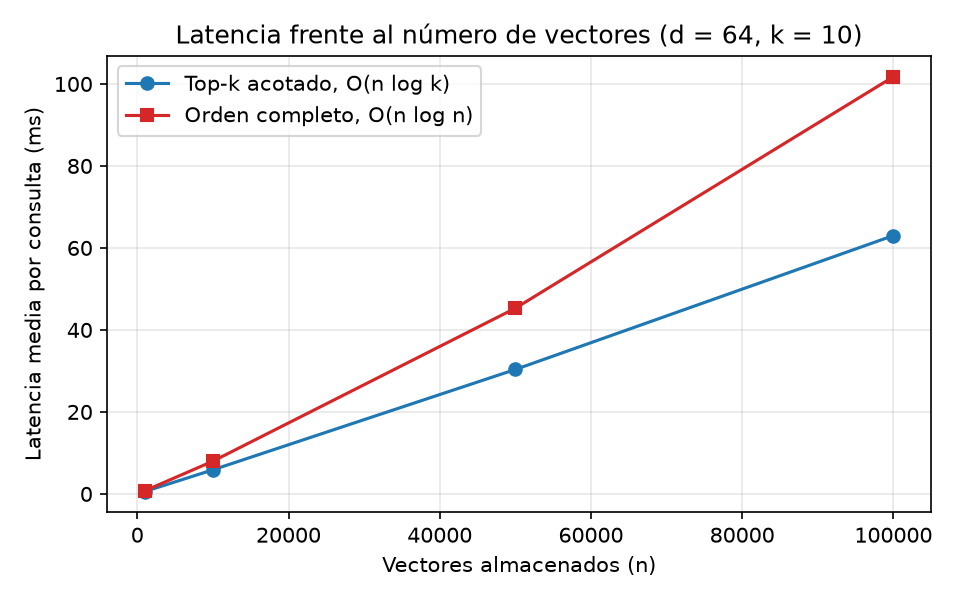
\includegraphics[width=0.82\textwidth]{../../experimentos/graficos/latencia_vs_vectores.png}
\caption{Latencia media frente al número de vectores.}
\label{fig:latencia-vectores}
\end{figure}

\begin{figure}[H]
\centering
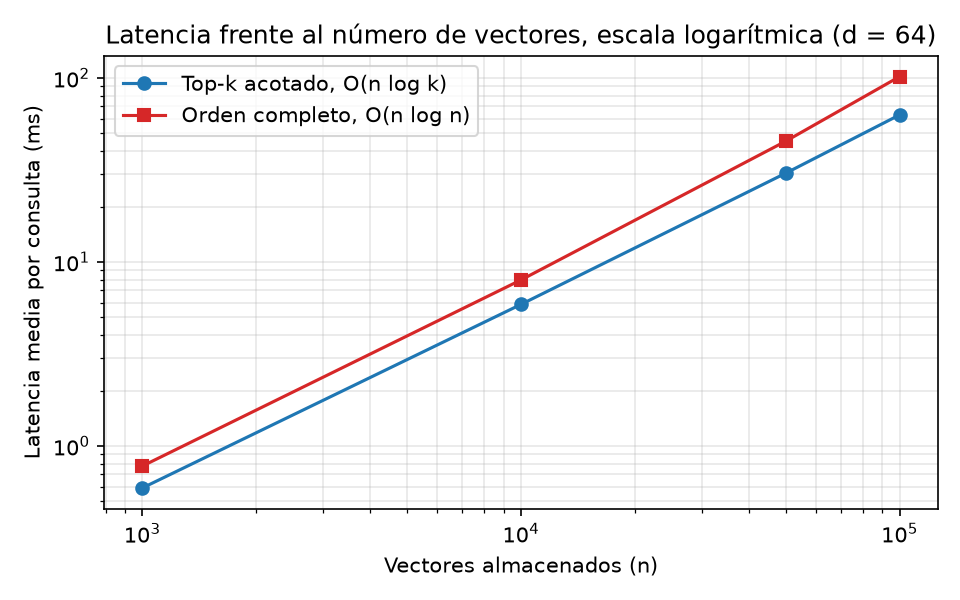
\includegraphics[width=0.82\textwidth]{../../experimentos/graficos/latencia_vs_vectores_log.png}
\caption{Latencia frente al número de vectores en escala doblemente logarítmica.}
\label{fig:latencia-vectores-log}
\end{figure}

\textbf{Tabla 4.} Aceleración de la selección Top-k, por número de
vectores y por dimensión.

\begin{longtable}[]{@{}C{0.21\textwidth}C{0.14\textwidth}C{0.03\textwidth}C{0.25\textwidth}C{0.14\textwidth}@{}}
\toprule\noalign{}
Vectores (\texttt{d\ =\ 64}, \texttt{k\ =\ 10}) & Aceleración & &
Dimensión (\texttt{n\ =\ 10\ 000}, \texttt{k\ =\ 10}) & Aceleración \\
\midrule\noalign{}
\endhead
\bottomrule\noalign{}
\endlastfoot
1 000 & 1,32× & & 16 & 1,67× \\
10 000 & 1,36× & & 32 & 1,56× \\
50 000 & 1,49× & & 128 & 1,22× \\
100 000 & 1,61× & & 256 & 1,19× \\
\end{longtable}

La tabla 4 muestra las dos tendencias opuestas que anticipaba H3: la
ventaja del Top-k \textbf{crece} con el número de vectores y
\textbf{decrece} con la dimensión.

\textbf{Tabla 5.} Latencia frente a la dimensionalidad
(\texttt{n\ =\ 10\ 000}, \texttt{k\ =\ 10}).

\begin{longtable}[]{@{}L{0.15\textwidth}*{6}{C{0.10\textwidth}}@{}}
\toprule\noalign{}
Estrategia & Dimensión & Media (ms) & p50 & p95 & p99 & Cons./s \\
\midrule\noalign{}
\endhead
\bottomrule\noalign{}
\endlastfoot
Top-k & 16 & 2,955 & 2,952 & 2,987 & 3,021 & 338 \\
Orden completo & 16 & 4,923 & 4,914 & 5,083 & 5,116 & 203 \\
Top-k & 32 & 3,694 & 3,683 & 3,789 & 3,834 & 271 \\
Orden completo & 32 & 5,758 & 5,754 & 5,901 & 5,913 & 174 \\
Top-k & 64 & 5,878 & 5,848 & 6,014 & 6,249 & 170 \\
Orden completo & 64 & 7,982 & 7,931 & 8,141 & 8,741 & 125 \\
Top-k & 128 & 10,378 & 10,320 & 10,763 & 10,769 & 96 \\
Orden completo & 128 & 12,656 & 12,615 & 13,187 & 13,244 & 79 \\
Top-k & 256 & 21,077 & 21,072 & 21,578 & 21,696 & 47 \\
Orden completo & 256 & 25,082 & 25,031 & 26,162 & 26,350 & 40 \\
\end{longtable}

La figura 4 representa la tabla 5. Multiplicar la dimensión por 16 ---de
16 a 256--- multiplica la latencia del Top-k por 7,1 y no por 16: el
crecimiento es sublineal, como anticipaba H2.

\begin{figure}[H]
\centering
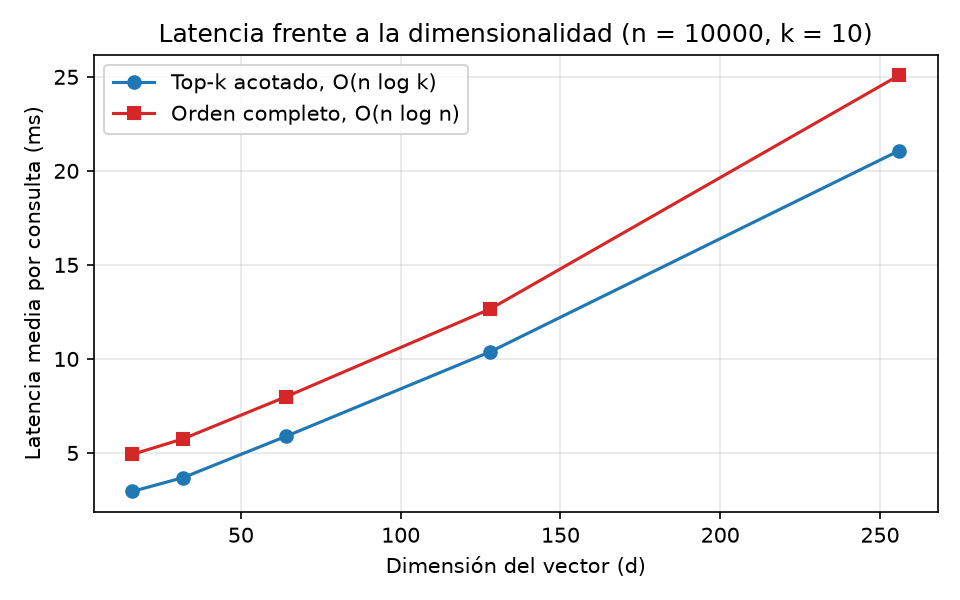
\includegraphics[width=0.82\textwidth]{../../experimentos/graficos/latencia_vs_dimension.png}
\caption{Latencia frente a la dimensión de los vectores.}
\label{fig:latencia-dimension}
\end{figure}

\textbf{Tabla 6.} Latencia frente a \texttt{k} (\texttt{n\ =\ 10\ 000},
\texttt{d\ =\ 64}).

\begin{longtable}[]{@{}C{0.10\textwidth}C{0.18\textwidth}C{0.10\textwidth}C{0.23\textwidth}C{0.10\textwidth}@{}}
\toprule\noalign{}
\texttt{k} & Top-k (ms) & σ & Orden completo (ms) & σ \\
\midrule\noalign{}
\endhead
\bottomrule\noalign{}
\endlastfoot
1 & 6,098 & 0,095 & 8,388 & 0,085 \\
5 & 5,915 & 0,095 & 8,267 & 0,523 \\
10 & 5,878 & 0,089 & 7,982 & 0,160 \\
20 & 6,100 & 0,110 & 8,753 & 0,877 \\
50 & 5,966 & 0,099 & 8,170 & 0,377 \\
\end{longtable}

La tabla 6 y la figura 5 muestran que \texttt{k} no produce ninguna
tendencia apreciable en el rango evaluado: la variación entre
\texttt{k\ =\ 1} y \texttt{k\ =\ 50} es del orden de la desviación
estándar de las propias medidas. H5 queda confirmada.

\begin{figure}[H]
\centering
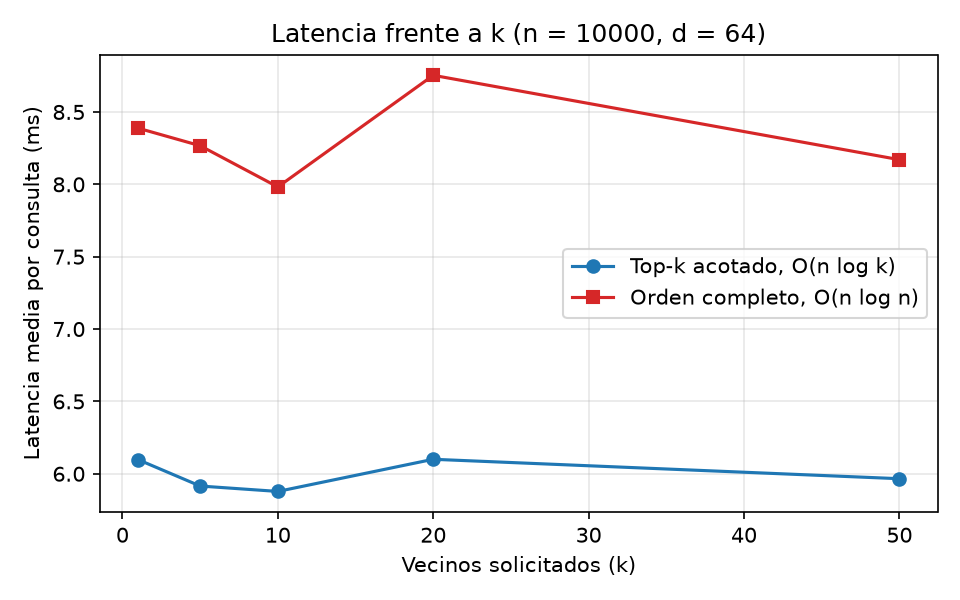
\includegraphics[width=0.82\textwidth]{../../experimentos/graficos/latencia_vs_k.png}
\caption{Latencia frente al número de vecinos solicitados, \texttt{k}.}
\label{fig:latencia-k}
\end{figure}

\begin{figure}[H]
\centering
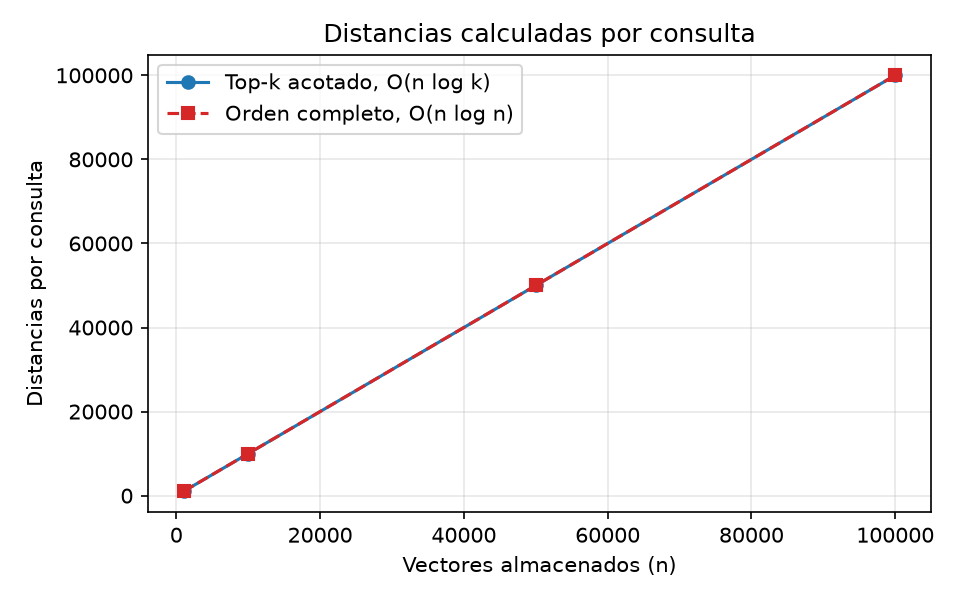
\includegraphics[width=0.82\textwidth]{../../experimentos/graficos/distancias_vs_vectores.png}
\caption{Distancias calculadas por consulta frente a \texttt{n}. Las series se superponen sobre $y=n$, pues ninguna estrategia poda el espacio.}
\label{fig:distancias-vectores}
\end{figure}

\subsubsection{6.8 Accesos a disco y comportamiento del
buffer}\label{68-accesos-a-disco-y-comportamiento-del-buffer}

\textbf{Tabla 7.} Entrada y salida por consulta (\texttt{d\ =\ 64},
\texttt{k\ =\ 10}). Los valores son idénticos en ambas estrategias, por
lo que se presenta una sola fila por volumen.

\begin{longtable}[]{@{}*{7}{C{0.125\textwidth}}@{}}
\toprule\noalign{}
Vectores & Páginas de datos & Lecturas físicas & Aciertos & Fallos &
Tasa de aciertos & Registros examinados \\
\midrule\noalign{}
\endhead
\bottomrule\noalign{}
\endlastfoot
1 000 & 86 & 67 & 1 000 & 67 & 0,9372 & 1 000 \\
10 000 & 745 & 710 & 10 000 & 710 & 0,9337 & 10 000 \\
50 000 & 3 698 & 3 567 & 50 000 & 3 567 & 0,9334 & 50 000 \\
100 000 & 7 398 & 7 139 & 100 000 & 7 139 & 0,9334 & 100 000 \\
\end{longtable}

La tabla 7 contiene tres observaciones. Primera, las lecturas físicas
por consulta equivalen prácticamente al número de páginas de datos: con
ocho marcos de buffer, cada consulta relee la tabla completa desde el
disco. Segunda, los accesos lógicos coinciden con el número de
registros, porque el iterador del montículo de tabla fija y libera la
página en cada registro que devuelve. Tercera, la tasa de aciertos se
estabiliza en 0,933, valor que no refleja localidad aprovechada sino la
relación entre registros por página y páginas: aproximadamente
\texttt{1\ −\ 1/14} con 14 registros por página.

\begin{figure}[H]
\centering
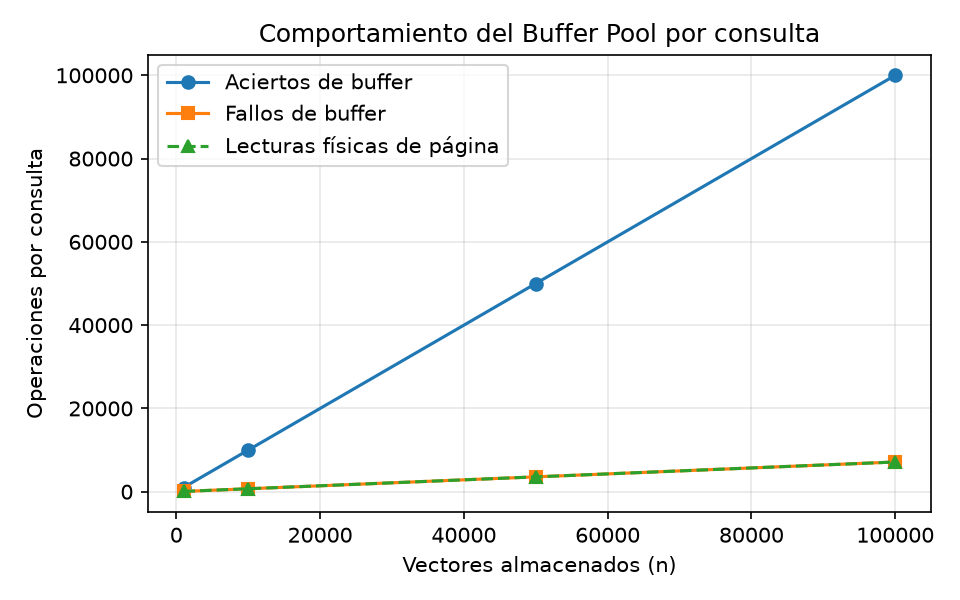
\includegraphics[width=0.82\textwidth]{../../experimentos/graficos/buffer_vs_vectores.png}
\caption{Aciertos, fallos y lecturas físicas por consulta frente a \texttt{n}.}
\label{fig:buffer-vectores}
\end{figure}

\begin{figure}[H]
\centering
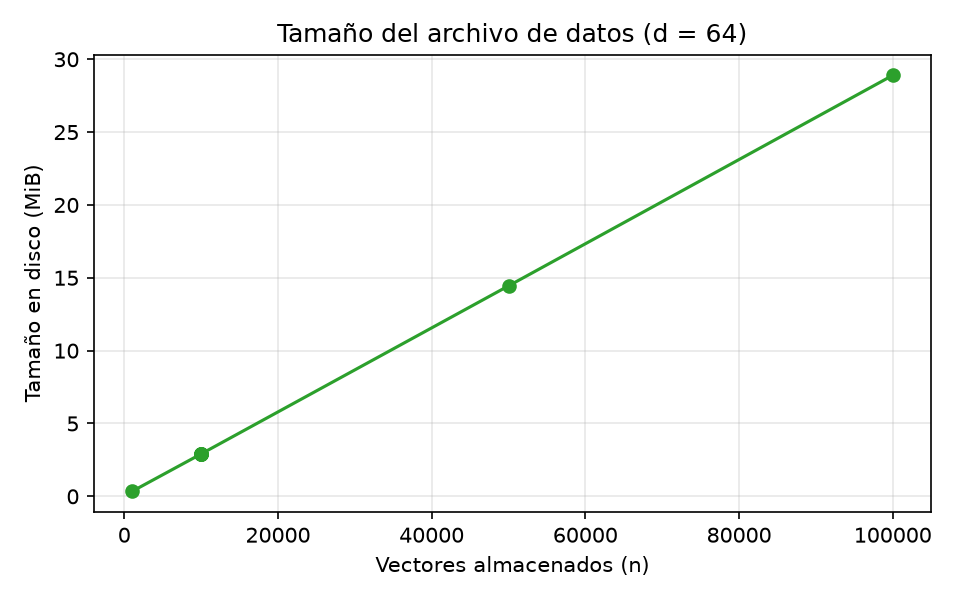
\includegraphics[width=0.82\textwidth]{../../experimentos/graficos/tamano_vs_vectores.png}
\caption{Tamaño del archivo de datos frente al número de vectores.}
\label{fig:tamano-vectores}
\end{figure}

\subsubsection{6.9 Búsqueda híbrida y método de
acceso}\label{69-buxfasqueda-huxedbrida-y-muxe9todo-de-acceso}

Dos propiedades adicionales se verifican en las pruebas automatizadas y
no requieren medición de tiempo, porque se comprueban con contadores
deterministas.

Con una tabla de 400 vectores y la consulta
\texttt{SELECT\ *\ FROM\ docs\ WHERE\ id\ \textless{}=\ 50\ NEAREST\ emb\ TO\ {[}...{]}\ LIMIT\ 5},
el plan construido es
\texttt{Projection\ →\ Knn\ →\ Filter\ →\ SequentialScan} y el número de
distancias calculadas es exactamente 50: el filtro por metadatos reduce
el conjunto de candidatos antes de que intervenga la aritmética
vectorial.

Sustituir el escaneo tupla a tupla por el escaneo por lotes deja el
resultado intacto ---mismas filas, mismo orden, mismo número de
distancias--- y cambia únicamente el número de fijaciones de página. El
ranking es, por tanto, independiente del método de acceso que lo
alimenta.

\subsubsection{6.10 Análisis
estadístico}\label{610-anuxe1lisis-estaduxedstico}

Con 30 observaciones por celda, la dispersión de la selección Top-k es
muy baja: su desviación estándar relativa oscila entre el 0,6 \% y el
1,5 \% de la media, y sus percentiles p95 y p99 se sitúan a menos del 3
\% de la mediana. El ordenamiento completo es sistemáticamente más
disperso ---hasta el 4,5 \% de desviación relativa en
\texttt{n\ =\ 50\ 000}, con un p99 un 18 \% por encima de su mediana---,
lo que resulta coherente con que asigne y libere memoria proporcional a
\texttt{n} en cada consulta.

Las diferencias entre estrategias son de uno a dos órdenes de magnitud
mayores que esta dispersión: en \texttt{n\ =\ 100\ 000} la separación
entre medias es de 38,7 ms frente a desviaciones de 0,4 y 1,8 ms. Los
intervalos no se solapan en ninguna configuración, de modo que la
diferencia observada no es atribuible al ruido de medición.

\begin{center}\rule{0.5\linewidth}{0.5pt}\end{center}

\subsection{7. Discusión}\label{7-discusiuxf3n}

\subsubsection{7.1 Respuesta a las preguntas de
investigación}\label{71-respuesta-a-las-preguntas-de-investigaciuxf3n}

\textbf{PI1.} El tiempo de consulta crece linealmente con el número de
vectores. El coeficiente medido para la selección Top-k con
\texttt{d\ =\ 64} es de aproximadamente 0,63 ms por cada mil vectores,
sostenido en dos órdenes de magnitud de volumen. Es el comportamiento
esperado de una búsqueda exhaustiva y, más que un resultado, es la
confirmación de que el sistema hace lo que dice hacer: sin índice
vectorial no existe poda posible y todo registro debe examinarse.

\textbf{PI2.} La dimensionalidad encarece la consulta de forma
sublineal. Ajustando un modelo lineal a los datos de la tabla 5 para la
selección Top-k se obtiene un componente fijo de aproximadamente 1,75 ms
por consulta, independiente de \texttt{d}, más unos 0,0755 ms por
dimensión. Ese componente fijo representa el 59 \% del coste con
\texttt{d\ =\ 16} y solo el 8 \% con \texttt{d\ =\ 256}: localizar la
ranura, deserializar el resto de la fila y atravesar el plan cuesta lo
mismo con vectores cortos que con vectores largos, y en dimensiones
bajas ese trabajo domina sobre la aritmética vectorial.

\textbf{PI3.} La selección Top-k acotada es entre 1,19 y 1,67 veces más
rápida que el ordenamiento completo, con dos tendencias sistemáticas y
opuestas. La ventaja crece con \texttt{n} ---de 1,32× con mil vectores a
1,61× con cien mil--- y decrece con \texttt{d} ---de 1,67× con dimensión
16 a 1,19× con dimensión 256.

\textbf{PI4.} El comportamiento de entrada y salida es idéntico en ambas
estrategias: mismas lecturas físicas, mismos aciertos y fallos, misma
tasa de aciertos, con diferencia nula en las cuatro configuraciones de
volumen. La ventaja del Top-k es íntegramente de cómputo y de memoria, y
no reduce en absoluto el tráfico con el disco. Es la respuesta más
importante del estudio en términos de honestidad: mejora la mitad del
coste que es aritmética, y no toca la mitad que es almacenamiento.

\subsubsection{7.2 Interpretación del comportamiento
observado}\label{72-interpretaciuxf3n-del-comportamiento-observado}

El resultado que mejor conecta la medición con la teoría es la evolución
opuesta de la aceleración frente a \texttt{n} y frente a \texttt{d}.
Ambos comportamientos se siguen del mismo modelo de coste. El tiempo de
una consulta puede escribirse como
\texttt{T\ ≈\ a·n·d\ +\ b·n·log\ R\ +\ c·n}, donde \texttt{R\ =\ k} para
la selección acotada y \texttt{R\ =\ n} para el ordenamiento completo, y
\texttt{c·n} recoge el coste por registro independiente de la dimensión.

Al aumentar \texttt{n} con \texttt{d} fijo, el término que distingue las
estrategias crece como \texttt{n\ log\ n} frente a \texttt{n\ log\ k},
mientras el resto crece linealmente: el peso relativo de la diferencia
aumenta, y la aceleración con ella. Al aumentar \texttt{d} con
\texttt{n} fijo, el término \texttt{a·n·d} crece y los demás no: la
diferencia entre estrategias se diluye en un coste aritmético común, y
la aceleración disminuye. Las dos tendencias medidas son, por tanto,
manifestaciones de una sola relación, y su concordancia con el modelo es
la evidencia más sólida de que lo que se está midiendo es realmente el
coste del ranking.

La independencia de \texttt{k} completa el cuadro. Entre
\texttt{k\ =\ 1} y \texttt{k\ =\ 50}, \texttt{log₂\ k} pasa de 0 a 5,6,
mientras \texttt{log₂\ n} vale 13,3 con diez mil vectores. La diferencia
predicha por el modelo queda por debajo de la dispersión de las medidas,
y es exactamente lo que se observa. Conviene subrayar la lectura
práctica: el coste de una búsqueda exhaustiva lo determina el tamaño de
la colección, no cuántos vecinos se pidan.

La superlinealidad del tiempo de carga de la tabla 1 tiene un origen
distinto y ajeno al aporte. La inserción en el montículo de tabla
intenta primero la última página y, si no cabe, recorre la cadena
buscando espacio liberado, comportamiento heredado del diseño original y
pensado para reutilizar huecos. Con \texttt{n} inserciones sobre una
cadena que crece hasta \texttt{p} páginas, el recorrido acumula del
orden de \texttt{n·p/2} fijaciones de página. Para
\texttt{n\ =\ 100\ 000} y \texttt{p\ =\ 7\ 398} eso arroja unos 3,7 ×
10⁸ accesos al buffer, que a un coste de doscientos nanosegundos por
acierto explica los 79 segundos medidos. Es una limitación real del
sistema, no una consecuencia de los vectores, aunque los vectores la
hacen visible al reducir los registros por página.

\subsubsection{7.3 Razones técnicas de las
diferencias}\label{73-razones-tuxe9cnicas-de-las-diferencias}

La selección acotada gana por tres mecanismos, en orden de importancia
decreciente. Primero, ordena \texttt{k} elementos en lugar de
\texttt{n}: con cien mil vectores y \texttt{k\ =\ 10}, unas 33
comparaciones de montículo frente a las aproximadamente 1,7 millones que
exige un \texttt{std::sort} de cien mil elementos. Segundo, la mayoría
de los candidatos se descartan con una única comparación contra la raíz
del montículo, sin entrar en la estructura; las pruebas documentan un
caso en el que solo diez de trescientos candidatos son admitidos.
Tercero, mantiene \texttt{O(k)} registros en memoria frente a
\texttt{O(n)}, lo que evita las reasignaciones sucesivas de un vector
que crece hasta contener la tabla completa, efecto que se aprecia en la
mayor dispersión y en los peores percentiles del ordenamiento completo.

Que las lecturas físicas coincidan exactamente en ambas estrategias no
es casual sino estructural: las dos consumen del mismo operador de
escaneo, que recorre la cadena de páginas del mismo modo. La estrategia
de ranking se aplica después de que la página haya sido leída, y por
tanto no puede influir en cuántas se leen. Ese es precisamente el
trabajo que un índice vectorial haría y que aquí no se hace.

\subsubsection{7.4 Relación con la complejidad
teórica}\label{74-relaciuxf3n-con-la-complejidad-teuxf3rica}

Los costes teóricos son \texttt{Θ(n·d\ +\ n\ log\ k)} para la propuesta
y \texttt{Θ(n·d\ +\ n\ log\ n)} para la línea base. Las mediciones son
consistentes con ellos en los tres aspectos comprobables: linealidad en
\texttt{n}, aceleración creciente en \texttt{n}, y aceleración
decreciente en \texttt{d}.

La discrepancia aparente entre la magnitud de la mejora asintótica y la
magnitud de la mejora medida ---un factor entre 1,2 y 1,7 donde la razón
\texttt{log\ n\ /\ log\ k} sugeriría más--- se explica por el término
\texttt{Θ(n·d)}, común a ambas, que domina el tiempo total. En la
configuración con dimensión 256, la aritmética vectorial supone más del
noventa por ciento del coste, de modo que ninguna mejora del ranking
puede superar un factor cercano a 1,1. Esto ilustra un principio
general: una mejora asintótica en un término no dominante produce una
mejora constante y modesta en el tiempo total.

\subsubsection{7.5 Ventajas de la
propuesta}\label{75-ventajas-de-la-propuesta}

La selección Top-k acotada es preferible en todas las configuraciones
evaluadas, sin ninguna contrapartida: es más rápida, más predecible en
su latencia de cola y usa memoria proporcional a \texttt{k} en lugar de
a \texttt{n}. Devuelve exactamente el mismo resultado, lo que se ha
verificado tanto en las doce configuraciones experimentales como
registro a registro en las pruebas automatizadas. La ventaja en memoria
es cualitativamente la más relevante: es la que determina si una
consulta sobre una colección grande puede ejecutarse en absoluto.

La integración con el motor aporta además dos capacidades que no
requieren código específico. El filtrado por metadatos previo al ranking
se obtiene por composición de operadores, y reduce el trabajo aritmético
en proporción directa a la selectividad del filtro. Y el ranking es
independiente del método de acceso, de modo que cualquier mejora futura
en el escaneo lo beneficia sin modificarlo.

\subsubsection{7.6 Limitaciones}\label{76-limitaciones}

La limitación fundamental es que la búsqueda sigue siendo exhaustiva. El
sistema no incorpora un índice vectorial, de modo que el coste crece
linealmente con la colección y la mejora obtenida es un factor
constante. Un índice IVF o HNSW cambiaría el orden de complejidad, que
es una diferencia de naturaleza distinta a la aquí medida.

Ninguna de las estrategias reduce el tráfico con el disco. Con ocho
marcos de buffer, cada consulta relee la tabla completa: en la
configuración de cien mil vectores, 7 139 lecturas físicas de página por
consulta. El sistema no implementa lectura anticipada, ni entrada y
salida asíncrona, ni almacenamiento columnar que permitiría leer solo la
columna vectorial en lugar de registros completos.

El acceso lógico por registro, y no por página, del iterador de tabla
multiplica los accesos al buffer. El sistema dispone de un escaneo por
lotes que fija cada página una sola vez, y las pruebas confirman que
puede alimentar el ranking sin alterar el resultado, pero la evaluación
de su efecto sobre las consultas vectoriales no forma parte de este
estudio.

Los volúmenes evaluados llegan a cien mil vectores de dimensión 64. Las
dimensiones típicas de los modelos de lenguaje actuales, entre 384 y
1536, no son abordables con holgura en un formato de página de 4 KiB, y
la dimensión máxima admitida es de 1000 componentes.

El sistema admite una sola tabla, no implementa transacciones, control
de concurrencia ni registro de escritura anticipada, y por tanto una
terminación abrupta puede perder las modificaciones no sincronizadas.

\subsubsection{7.7 Amenazas a la
validez}\label{77-amenazas-a-la-validez}

\textbf{Validez interna.} Ambas estrategias se ejecutan en el mismo
proceso, sobre el mismo archivo, con la misma configuración de buffer y
con vectores de consulta idénticos generados desde una semilla fija.
Comparten la función que calcula las puntuaciones, lo que garantiza que
la aritmética medida sea la misma. Se descarta una consulta de
calentamiento por ronda para no imputar a la primera medición el coste
de poblar el buffer. La amenaza residual es el orden de ejecución: la
ronda del Top-k precede siempre a la del ordenamiento completo, de modo
que un efecto sistemático del estado de la caché del procesador
favorecería a la primera. La estabilidad de las medianas entre las
treinta repeticiones sugiere que el efecto es pequeño, pero no se ha
controlado alternando el orden.

\textbf{Validez externa.} Los vectores son sintéticos y uniformes. Los
\emph{embeddings} reales presentan estructura de agrupamiento y normas
no uniformes, que afectarían a la distribución de distancias y, por
tanto, a la frecuencia con que un candidato mejora la raíz del
montículo. En consecuencia, la aceleración medida es una estimación para
datos sin estructura, y con datos agrupados podría diferir: si los
vecinos aparecen temprano en el recorrido, el montículo rechaza más
candidatos y la ventaja aumentaría. Las conclusiones sobre las
tendencias frente a \texttt{n}, \texttt{d} y \texttt{k} son más robustas
que las cifras concretas de aceleración, porque se derivan del modelo de
coste y no de la distribución de los datos. Las mediciones proceden
además de una única máquina y una única compilación.

\textbf{Validez de constructo.} Las magnitudes medidas corresponden a lo
que pretenden medir: las distancias se cuentan en el punto exacto del
cálculo; los aciertos y fallos, en la función de obtención de página del
administrador de buffer; y las lecturas físicas, solo cuando se invoca
la lectura del gestor de disco. La latencia se mide con un reloj
monótono e incluye el análisis sintáctico de la sentencia, que en una
consulta de proximidad implica interpretar un literal de \texttt{d}
componentes. Esa inclusión sobrestima ligeramente el coste de la
búsqueda, y lo hace más para dimensiones altas: parte del crecimiento
con \texttt{d} de la tabla 5 corresponde al analizador y no al ranking.
No se ha aislado esa fracción, lo que constituye una amenaza reconocida
a la interpretación de PI2.

\textbf{Validez de las conclusiones.} Las diferencias entre estrategias
superan la dispersión de las medidas en uno o dos órdenes de magnitud y
son consistentes en las doce configuraciones, por lo que no son
atribuibles al azar. Las afirmaciones sobre tendencias se apoyan en
cuatro puntos para \texttt{n} y cinco para \texttt{d}, un número
reducido: se presentan como consistentes con el modelo de coste, no como
un ajuste estadístico. No se han aplicado pruebas de significación
formales, lo que sería el paso natural con más repeticiones.

\begin{center}\rule{0.5\linewidth}{0.5pt}\end{center}

\subsection{8. Conclusiones}\label{8-conclusiones}

Este trabajo incorporó búsqueda exacta por similitud vectorial a un SGBD
didáctico paginado, integrando un tipo de dato \texttt{VECTOR(d)} en el
formato binario existente, tres métricas de distancia y similitud, y una
consulta de los \texttt{k} vecinos más cercanos dentro del motor de
operadores físicos del sistema. Se evaluaron dos estrategias de ranking
sobre datos, consultas y configuración idénticos, con 720 observaciones
a lo largo de doce configuraciones.

Respecto del objetivo general, la integración es funcional y
verificable: los vectores persisten en las mismas páginas ranuradas que
los registros convencionales, se leen a través del mismo administrador
de buffer, y una consulta de proximidad compone con el filtrado por
metadatos sin código específico. Trescientas dieciséis pruebas
automatizadas, ejecutadas también bajo detectores de errores de memoria
y de comportamiento indefinido, respaldan esa afirmación.

Sobre las preguntas de investigación, el coste de una consulta crece
linealmente con el número de vectores, como corresponde a una búsqueda
sin poda, y de forma sublineal con la dimensión, porque una parte del
coste por registro es independiente de ella y llega a representar cerca
del sesenta por ciento en dimensiones bajas. La selección Top-k acotada
supera al ordenamiento completo en todas las configuraciones evaluadas,
con una ventaja que crece al aumentar la colección y se diluye al
aumentar la dimensión; ambas tendencias se derivan del mismo modelo de
coste y su concordancia con él es el resultado más sólido del estudio.
El número de vecinos solicitado no produjo efecto apreciable en el rango
evaluado. Finalmente, el comportamiento de entrada y salida resultó
idéntico en las dos estrategias: la mejora es exclusivamente de cómputo
y de memoria, y no reduce el tráfico con el disco.

La propuesta rinde mejor cuando la colección es grande, la dimensión
moderada y \texttt{k} pequeño frente a \texttt{n}, que es el régimen
habitual de una consulta de recuperación. Su ventaja más valiosa no es
la de tiempo, moderada, sino la de espacio: mantener \texttt{k}
candidatos en lugar de \texttt{n} es lo que determina si una consulta
sobre una colección grande puede ejecutarse.

La limitación que domina todas las demás es que la búsqueda permanece
exhaustiva. Una mejora del ranking actúa sobre un término que no domina
el coste total, y por eso produce un factor constante y modesto en lugar
de un cambio de orden. Reducir el coste de forma cualitativa exige no
examinar todos los vectores, es decir un índice vectorial.

Las líneas de trabajo futuro técnicamente viables sobre este sistema,
ninguna de las cuales forma parte de la implementación evaluada, son las
siguientes. Un índice IVF-Flat, con centroides obtenidos por k-means y
persistidos en páginas propias accedidas mediante el administrador de
buffer, es la de mejor relación entre coste de implementación y efecto,
y permitiría además evaluar \texttt{Recall@k} frente a la búsqueda
exacta que este trabajo ya proporciona como referencia. Un índice HNSW
ofrecería mejor latencia a cambio de una estructura de grafo persistente
considerablemente más compleja. La cuantización de producto reduciría
los bytes por vector y con ellos las páginas a leer, que es el cuello de
botella identificado en la sección 7.6. Un almacenamiento columnar para
la columna vectorial permitiría leer solo los vectores en lugar de
registros completos. La evaluación del escaneo por lotes aplicado a
consultas vectoriales es inmediata, puesto que ambos componentes ya
existen y su compatibilidad está verificada. Por último, evaluar el
sistema con \emph{embeddings} reales permitiría comprobar en qué medida
la estructura de agrupamiento de los datos altera las aceleraciones
medidas sobre datos uniformes.

\begin{center}\rule{0.5\linewidth}{0.5pt}\end{center}

\subsection{9. Referencias}\label{9-referencias}

{[}1{]} J. L. Bentley, \enquote{Multidimensional binary search trees used for
associative searching}, \emph{Communications of the ACM}, vol. 18, no.
9, pp. 509--517, 1975.

{[}2{]} A. Guttman, \enquote{R-trees: A dynamic index structure for spatial
searching}, in \emph{Proc. ACM SIGMOD International Conference on
Management of Data}, 1984, pp. 47--57.

{[}3{]} R. Weber, H.-J. Schek, and S. Blott, \enquote{A quantitative analysis
and performance study for similarity-search methods in high-dimensional
spaces}, in \emph{Proc. 24th International Conference on Very Large Data
Bases (VLDB)}, 1998, pp. 194--205.

{[}4{]} K. Beyer, J. Goldstein, R. Ramakrishnan, and U. Shaft, \enquote{When is
\textquotesingle nearest neighbor\textquotesingle{} meaningful?}, in
\emph{Proc. 7th International Conference on Database Theory (ICDT)},
1999, pp. 217--235.

{[}5{]} P. Indyk and R. Motwani, \enquote{Approximate nearest neighbors: Towards
removing the curse of dimensionality}, in \emph{Proc. 30th Annual ACM
Symposium on Theory of Computing (STOC)}, 1998, pp. 604--613.

{[}6{]} A. Gionis, P. Indyk, and R. Motwani, \enquote{Similarity search in high
dimensions via hashing}, in \emph{Proc. 25th International Conference on
Very Large Data Bases (VLDB)}, 1999, pp. 518--529.

{[}7{]} H. Jégou, M. Douze, and C. Schmid, \enquote{Product quantization for
nearest neighbor search}, \emph{IEEE Transactions on Pattern Analysis
and Machine Intelligence}, vol. 33, no. 1, pp. 117--128, 2011.

{[}8{]} Y. A. Malkov and D. A. Yashunin, \enquote{Efficient and robust
approximate nearest neighbor search using hierarchical navigable small
world graphs}, \emph{IEEE Transactions on Pattern Analysis and Machine
Intelligence}, vol. 42, no. 4, pp. 824--836, 2020.

{[}9{]} J. Johnson, M. Douze, and H. Jégou, \enquote{Billion-scale similarity
search with GPUs}, \emph{IEEE Transactions on Big Data}, vol. 7, no. 3,
pp. 535--547, 2021.

{[}10{]} M. Douze, A. Guzhva, C. Deng, J. Johnson, G. Szilvasy, P.-E.
Mazaré, M. Lomeli, L. Hosseini, and H. Jégou, \enquote{The Faiss library}, arXiv
preprint arXiv:2401.08281, 2024.

{[}11{]} J. Wang, X. Yi, R. Guo, H. Jin, P. Xu, S. Li, X. Wang, X. Guo,
C. Li, X. Xu, K. Yu, Y. Yuan, Y. Zou, J. Long, Y. Cai, Z. Li, Z. Zhang,
Y. Mo, J. Gu, R. Jiang, Y. Wei, and C. Xie, \enquote{Milvus: A purpose-built
vector data management system}, in \emph{Proc. ACM SIGMOD International
Conference on Management of Data}, 2021, pp. 2614--2627.

{[}12{]} pgvector contributors, \enquote{pgvector: Open-source vector similarity
search for PostgreSQL}. {[}Online{]}. Available:
\url{https://github.com/pgvector/pgvector}

{[}13{]} Qdrant, \enquote{Qdrant documentation}. {[}Online{]}. Available:
\url{https://qdrant.tech/documentation/}

{[}14{]} G. Graefe, \enquote{Query evaluation techniques for large databases},
\emph{ACM Computing Surveys}, vol. 25, no. 2, pp. 73--169, 1993.

{[}15{]} G. Graefe, \enquote{Volcano --- an extensible and parallel query
evaluation system}, \emph{IEEE Transactions on Knowledge and Data
Engineering}, vol. 6, no. 1, pp. 120--135, 1994.

{[}16{]} P. A. Boncz, M. Zukowski, and N. Nes, \enquote{MonetDB/X100:
Hyper-pipelining query execution}, in \emph{Proc. 2nd Biennial
Conference on Innovative Data Systems Research (CIDR)}, 2005.

{[}17{]} W. Effelsberg and T. Haerder, \enquote{Principles of database buffer
management}, \emph{ACM Transactions on Database Systems}, vol. 9, no. 4,
pp. 560--595, 1984.

{[}18{]} A. Silberschatz, H. F. Korth, and S. Sudarshan, \emph{Database
System Concepts}, 7th ed. New York, NY, USA: McGraw-Hill, 2019.

{[}19{]} R. Ramakrishnan and J. Gehrke, \emph{Database Management
Systems}, 3rd ed. New York, NY, USA: McGraw-Hill, 2003.

{[}20{]} M. Aumüller, E. Bernhardsson, and A. Faithfull,
\enquote{ANN-Benchmarks: A benchmarking tool for approximate nearest neighbor
algorithms}, \emph{Information Systems}, vol. 87, 2020.

\begin{quote}
Los datos bibliográficos que no han podido verificarse contra la fuente
original ---en particular números de página y de volumen de algunas
actas de congreso--- se enumeran en
\texttt{docs/referencias\_pendientes.md} para su comprobación antes de
un envío real.
\end{quote}

\begin{center}\rule{0.5\linewidth}{0.5pt}\end{center}

\begin{landscape}
\subsection{Anexo A. Trazabilidad entre afirmaciones y
código}\label{anexo-a-trazabilidad-entre-afirmaciones-y-cuxf3digo}

\begin{longtable}[]{@{}L{0.20\linewidth}L{0.18\linewidth}L{0.24\linewidth}L{0.32\linewidth}@{}}
\toprule\noalign{}
Afirmación técnica & Evidencia & Archivo & Clase o función \\
\midrule\noalign{}
\endhead
\bottomrule\noalign{}
\endlastfoot
Existe un tipo de columna vectorial & Tercer valor del enumerado de
tipos & \texttt{include/minidb/common/types.hpp} &
\texttt{ColumnType::kVector} \\
Un vector es un arreglo de \texttt{float} de 32 bits & Alias de tipo y
variante de valor & \texttt{include/minidb/common/value.hpp} &
\texttt{Vector}, \texttt{Value} \\
Los vectores se serializan en IEEE 754 \emph{little-endian} & Escritura
mediante \texttt{std::bit\_cast} & \texttt{src/common/serialization.cpp}
& \texttt{serialization::WriteF32}, \texttt{serialization::ReadF32} \\
Los vectores persisten en páginas ranuradas & Caso vectorial de la
serialización de registros & \texttt{src/storage/record.cpp} &
\texttt{Record::SerializeTo}, \texttt{Record::DeserializeFrom} \\
La dimensión es fija y se valida & Comprobación por columna &
\texttt{src/storage/record.cpp} & \texttt{Record::Validate} \\
Ningún registro válido excede una página & Comprobación del registro más
ancho & \texttt{src/catalog/schema.cpp} & \texttt{Schema::Schema} \\
El catálogo rechaza tipos de columna desconocidos & Validación del byte
de tipo al recargar & \texttt{src/catalog/catalog.cpp} &
\texttt{Catalog::Load} \\
Distancia euclidiana y su cuadrado & Función de un solo recorrido &
\texttt{src/vector/distance.cpp} &
\texttt{vector\_metrics::SquaredEuclideanDistance} \\
Similitud y distancia coseno distinguidas & Dos funciones separadas &
\texttt{src/vector/distance.cpp} & \texttt{CosineSimilarity},
\texttt{CosineDistance} \\
Producto punto & Función de un solo recorrido &
\texttt{src/vector/distance.cpp} &
\texttt{vector\_metrics::DotProduct} \\
El vector nulo no produce \texttt{NaN} & Caso explícito de norma cero &
\texttt{src/vector/distance.cpp} &
\texttt{vector\_metrics::CosineSimilarity} \\
Las dimensiones incompatibles se rechazan & Comprobación previa al
cálculo & \texttt{src/vector/distance.cpp} &
\texttt{RequireSameDimension} \\
Menor puntuación es siempre más cercano & Cuadrado y negación según
métrica & \texttt{src/vector/distance.cpp} &
\texttt{vector\_metrics::RankingScore} \\
Selección Top-k con montículo acotado & Comparación contra la raíz &
\texttt{src/execution/knn\_operators.cpp} &
\texttt{KnnScanOperator::Open} \\
Línea base con orden completo de \texttt{n} & Conserva todos y ordena &
\texttt{src/execution/knn\_operators.cpp} &
\texttt{KnnFullSortOperator::Open} \\
Los empates se resuelven por clave primaria & Comparador con desempate &
\texttt{src/execution/knn\_operators.cpp} &
\texttt{KnnScanOperator::Closer} \\
\texttt{k\ =\ 0} no recorre la tabla & Salida temprana &
\texttt{src/execution/knn\_operators.cpp} &
\texttt{KnnScanOperator::Open} \\
La dimensión de la consulta se valida al planificar & Comprobación en el
constructor & \texttt{src/execution/knn\_operators.cpp} &
\texttt{KnnScanOperator::KnnScanOperator} \\
El plan es \texttt{Projection(Knn(Filter?(Scan)))} & Construcción del
plan & \texttt{src/execution/execution\_engine.cpp} &
\texttt{ExecutionEngine::BuildPlan} \\
La estrategia de ranking es conmutable & Interruptor del planificador &
\texttt{include/minidb/execution/execution\_engine.hpp} &
\texttt{ExecutionEngine::SetTopKEnabled} \\
Se cuentan las distancias calculadas & Contador en el punto del cálculo
& \texttt{include/minidb/execution/physical\_operator.hpp} &
\texttt{PhysicalOperator::CountDistance} \\
Se cuentan los candidatos retenidos & Contador en la admisión &
\texttt{include/minidb/execution/physical\_operator.hpp} &
\texttt{PhysicalOperator::CountCandidate} \\
Se distinguen acierto, fallo y lectura física & Contadores separados &
\texttt{src/buffer/buffer\_pool\_manager.cpp} &
\texttt{BufferPoolManager::FetchPage} \\
La latencia se mide con reloj monótono & Medición alrededor de la
sentencia & \texttt{src/database/database.cpp} &
\texttt{Database::Execute} \\
Las consultas de prueba son reproducibles & Generador con semilla fija &
\texttt{src/main.cpp} & \texttt{MakeQueryVectors} \\
Los CSV se generan sin intervención manual & Exportación desde la
interfaz & \texttt{src/main.cpp} & \texttt{RunKnnCsv} \\
Las métricas coinciden con valores de forma cerrada & 19 casos de prueba
& \texttt{tests/distance\_test.cpp} & \texttt{DistanceTest} \\
Las dos estrategias devuelven lo mismo & Comparación fila a fila &
\texttt{tests/knn\_test.cpp} &
\texttt{KnnEquivalenceTest.BothStrategiesReturnIdenticalResults} \\
El filtro reduce las distancias calculadas & Contador tras un
\texttt{WHERE} & \texttt{tests/knn\_test.cpp} &
\texttt{KnnEquivalenceTest.AWhereClauseFiltersBeforeTheRanking} \\
\end{longtable}
\end{landscape}

\begin{landscape}
\subsection{Anexo B. Estado de las
funcionalidades}\label{anexo-b-estado-de-las-funcionalidades}

\begin{longtable}[]{@{}L{0.18\linewidth}L{0.12\linewidth}L{0.28\linewidth}L{0.36\linewidth}@{}}
\toprule\noalign{}
Funcionalidad & Estado & Evidencia & Observación \\
\midrule\noalign{}
\endhead
\bottomrule\noalign{}
\endlastfoot
Gestor de almacenamiento & Implementado &
\texttt{src/storage/disk\_manager.cpp} & Páginas fijas de 4096 B en un
único archivo binario \\
Administrador de páginas & Implementado &
\texttt{src/storage/table\_page.cpp} & Página ranurada con
compactación \\
Administrador de buffer & Implementado &
\texttt{src/buffer/buffer\_pool\_manager.cpp} & Marcos fijos, LRU,
escritura al desalojar \\
Catálogo & Implementado & \texttt{src/catalog/catalog.cpp} & Persistido
en la página 1; valida el tipo al recargar \\
Tipo de dato vectorial & Implementado &
\texttt{include/minidb/common/types.hpp} & \texttt{VECTOR(d)} con
\texttt{1\ ≤\ d\ ≤\ 1000} \\
Serialización de vectores & Implementado &
\texttt{src/common/serialization.cpp} & \texttt{2\ +\ 4d} bytes, IEEE
754 \emph{little-endian} \\
Persistencia de vectores & Implementado & \texttt{tests/knn\_test.cpp} &
Verificada bit a bit tras cerrar y reabrir \\
Métricas de similitud & Implementado & \texttt{src/vector/distance.cpp}
& Euclidiana, coseno y producto punto \\
Consulta k-NN & Implementado & \texttt{src/execution/knn\_operators.cpp}
& Exacta y exhaustiva \\
Búsqueda secuencial & Implementado &
\texttt{src/execution/operators.cpp} & Alimenta el ranking \\
Índice vectorial & \textbf{Ausente} & --- & No se encontró evidencia
porque no existe; se propone como trabajo futuro \\
Búsqueda aproximada y \texttt{Recall@k} & \textbf{Ausente} & --- & Sin
búsqueda aproximada no hay pérdida que cuantificar \\
Selector Top-k & Implementado &
\texttt{src/execution/knn\_operators.cpp} & Montículo acotado de tamaño
\texttt{k} \\
Instrumentación de tiempo & Implementado &
\texttt{src/database/database.cpp} & Reloj monótono por sentencia \\
Instrumentación de aciertos y fallos & Implementado &
\texttt{src/buffer/buffer\_pool\_manager.cpp} & Distingue acceso lógico
de lectura física \\
Instrumentación de distancias & Implementado &
\texttt{include/minidb/execution/physical\_operator.hpp} & Contada en el
punto del cálculo \\
Memoria máxima utilizada & \textbf{Ausente} & --- & No se instrumentó;
el espacio se mide indirectamente por candidatos retenidos \\
Pruebas automatizadas & Implementado & \texttt{tests/} & 316 casos,
verdes también bajo saneadores \\
Benchmarks & Implementado & \texttt{src/main.cpp},
\texttt{experimentos/scripts/} & Órdenes \texttt{.knnbench} y
\texttt{.knncsv} \\
\end{longtable}
\end{landscape}

\begin{landscape}
\subsection{Anexo C. Matriz
experimental}\label{anexo-c-matriz-experimental}

\begin{longtable}[]{@{}L{0.12\linewidth}L{0.11\linewidth}L{0.11\linewidth}L{0.18\linewidth}L{0.22\linewidth}C{0.10\linewidth}L{0.10\linewidth}@{}}
\toprule\noalign{}
Experimento & Línea base & Propuesta & Datos & Orden & Repeticiones &
Salida \\
\midrule\noalign{}
\endhead
\bottomrule\noalign{}
\endlastfoot
E1: efecto de \texttt{n} & Orden completo & Top-k acotado &
\texttt{n\ ∈\ \{1000,\ 10⁴,\ 5×10⁴,\ 10⁵\}}, \texttt{d\ =\ 64},
\texttt{k\ =\ 10} &
\texttt{.knncsv\ \textless{}ruta\textgreater{}\ 10\ 30} & 30 + 1
calentamiento & \texttt{resultados\_crudos.csv} \\
E2: efecto de \texttt{d} & Orden completo & Top-k acotado &
\texttt{n\ =\ 10⁴}, \texttt{d\ ∈\ \{16,\ 32,\ 64,\ 128,\ 256\}},
\texttt{k\ =\ 10} &
\texttt{.knncsv\ \textless{}ruta\textgreater{}\ 10\ 30} & 30 + 1 &
ídem \\
E3: efecto de \texttt{k} & Orden completo & Top-k acotado &
\texttt{n\ =\ 10⁴}, \texttt{d\ =\ 64},
\texttt{k\ ∈\ \{1,\ 5,\ 10,\ 20,\ 50\}} &
\texttt{.knncsv\ \textless{}ruta\textgreater{}\ \textless{}k\textgreater{}\ 30}
& 30 + 1 & ídem \\
E4: entrada y salida & Orden completo & Top-k acotado & Igual que E1 &
ídem & 30 + 1 & \texttt{metricas\_io.csv} \\
E5: exactitud & Orden completo & Top-k acotado & Las doce
configuraciones & \texttt{procesar\_resultados.py} & --- &
\texttt{exactitud.csv} \\
E6: validación funcional & --- & --- & Casos calculables a mano &
\texttt{ctest -R "Distance|Knn|Vector"} & --- & Salida de CTest \\
\end{longtable}
\end{landscape}

\subsection{Anexo D. Órdenes de
reproducción}\label{anexo-d-uxf3rdenes-de-reproducciuxf3n}

\begin{Shaded}
\begin{Highlighting}[]
\CommentTok{\# 1. Compilar en modo Release}
\FunctionTok{cmake} \AttributeTok{{-}S}\NormalTok{ . }\AttributeTok{{-}B}\NormalTok{ build{-}release }\AttributeTok{{-}G}\NormalTok{ Ninja }\AttributeTok{{-}DCMAKE\_BUILD\_TYPE}\OperatorTok{=}\NormalTok{Release}
\FunctionTok{cmake} \AttributeTok{{-}{-}build}\NormalTok{ build{-}release }\AttributeTok{{-}j}\StringTok{"}\VariableTok{$(}\FunctionTok{nproc}\VariableTok{)}\StringTok{"}

\CommentTok{\# 2. Ejecutar las pruebas, incluida la validación funcional}
\ExtensionTok{ctest} \AttributeTok{{-}{-}test{-}dir}\NormalTok{ build{-}release }\AttributeTok{{-}{-}output{-}on{-}failure}

\CommentTok{\# 3. Comprobar también bajo saneadores de memoria y comportamiento indefinido}
\FunctionTok{cmake} \AttributeTok{{-}S}\NormalTok{ . }\AttributeTok{{-}B}\NormalTok{ build{-}sanitize }\AttributeTok{{-}G}\NormalTok{ Ninja }\AttributeTok{{-}DCMAKE\_BUILD\_TYPE}\OperatorTok{=}\NormalTok{Debug }\DataTypeTok{\textbackslash{}}
      \AttributeTok{{-}DMINIDB\_ENABLE\_SANITIZERS}\OperatorTok{=}\NormalTok{ON}
\FunctionTok{cmake} \AttributeTok{{-}{-}build}\NormalTok{ build{-}sanitize }\AttributeTok{{-}j}\StringTok{"}\VariableTok{$(}\FunctionTok{nproc}\VariableTok{)}\StringTok{"}
\ExtensionTok{ctest} \AttributeTok{{-}{-}test{-}dir}\NormalTok{ build{-}sanitize }\AttributeTok{{-}{-}output{-}on{-}failure}

\CommentTok{\# 4. Generar los datos de un caso concreto y cargarlos}
\ExtensionTok{python3}\NormalTok{ experimentos/scripts/generar\_vectores.py }\AttributeTok{{-}{-}vectores}\NormalTok{ 10000 }\AttributeTok{{-}{-}dimension}\NormalTok{ 64 }\DataTypeTok{\textbackslash{}}
    \OperatorTok{\textgreater{}}\NormalTok{ /tmp/carga.sql}
\ExtensionTok{./build{-}release/minidb}\NormalTok{ /tmp/docs.db /dev/null }\OperatorTok{\textless{}}\NormalTok{ /tmp/carga.sql}

\CommentTok{\# 5. Ejecutar una consulta de vecinos más cercanos de forma interactiva}
\ExtensionTok{./build{-}release/minidb}\NormalTok{ /tmp/docs.db}
\CommentTok{\#   SELECT * FROM docs NEAREST emb TO [0.5, 0.5, ...] USING COSINE LIMIT 5;}
\CommentTok{\#   .topk off      {-}{-} cambia a la línea base de ordenamiento completo}
\CommentTok{\#   .knnbench 10 30}

\CommentTok{\# 6. Ejecutar la matriz experimental completa (regenera los CSV)}
\ExtensionTok{python3}\NormalTok{ experimentos/scripts/ejecutar\_benchmarks.py}

\CommentTok{\# 7. Agregar los resultados en las tablas del artículo}
\ExtensionTok{python3}\NormalTok{ experimentos/scripts/procesar\_resultados.py}

\CommentTok{\# 8. Generar las figuras}
\ExtensionTok{python3}\NormalTok{ experimentos/scripts/generar\_graficos.py}
\end{Highlighting}
\end{Shaded}

Ninguna de las órdenes anteriores edita un CSV a mano: los archivos de
\texttt{experimentos/resultados/} se regeneran por completo en cada
ejecución del paso 6.

\end{document}
